\documentclass[
11pt,%
tightenlines,%
twoside,%
onecolumn,%
nofloats,%
nobibnotes,%
nofootinbib,%
superscriptaddress,%
noshowpacs,%
centertags]%
{revtex4}
\usepackage{ljm}
\usepackage{listings}
\usepackage[utf8]{inputenc}
\usepackage[russian]{babel}

\lstset{
language=C++,
basewidth=0.5em,
xleftmargin=45pt,
xrightmargin=45pt,
basicstyle=\small\ttfamily,
keywordstyle=\bfseries\underbar,
numbers=left,
numberstyle=\tiny,
stepnumber=1,
numbersep=10pt,
showspaces=false,
showstringspaces=false,
showtabs=false,
frame=trBL,
tabsize=2,
captionpos=t,
breaklines=true,
breakatwhitespace=false,
escapeinside={\%*}{*)}
}

\begin{document}

\titlerunning{Computational mesh evolution}
\authorrunning{Meshcheryakov et al.}

\title{Evolution of the surface computational mesh in the ice accretion process}

\author{\firstname{A.~O.}~\surname{Meshcheryakov}}
\email[E-mail: ]{alex2501@jscc.ru}
\affiliation{Joint Supercomputer Center of the Russian Academy of Sciences -- branch of Scientific Research Institute of System Analysis of the Russian Academy of Sciences, Leninsky prospect 32a, Moscow, 119334, Russia}

\author{\firstname{A.~A.}~\surname{Rybakov}}
\email[E-mail: ]{rybakov@jscc.ru}
\affiliation{Joint Supercomputer Center of the Russian Academy of Sciences -- branch of Scientific Research Institute of System Analysis of the Russian Academy of Sciences, Leninsky prospect 32a, Moscow, 119334, Russia}

\firstcollaboration{(Submitted by TODO)} % Add if you know submitter.
%\lastcollaboration{ }

\received{TODO}

\begin{abstract}
%Задача моделирования обледенения поверхности обтекаемого тела является критической для обеспечения безопасности полетов в условия ледообразования.
The task of modeling the ice accretion of the surface of a streamlined body is critical for ensuring flight safety in conditions of ice formation.
%Формирование ледяных наростов на несущих частях и элементах силовых установок летальных аппаратов может существенно влиять на летные характеристики.
The formation of ice growths on the bearing parts and elements of the power systems of aircraft can significantly affect the flight characteristics.
%Сам процесс ледообразования является комплексным.
The process of ice formation itself is complex.
%Для получения качественной картины профиля ледяного нароста необходимо учитывать множество физических процессов, включая динамику газа, теплопроводность, динамику капель, выпадающих на поверхность, течение жидкости по поверхности.
To obtain a qualitative picture of the ice buildup profile, it is necessary to take into account many physical processes, including gas dynamics, thermal conductivity, the dynamics of drops falling to the surface, and the flow of liquid over the surface.
%Расчет ледяного покрова должен выполняться итерационно, так как образующийся лед существенно влияет на газодинамические характеристики, которые должны пересчитываться с ростом льда.
The calculation of the ice cover must be performed iteratively, since the resulting ice significantly affects the gas-dynamic characteristics, which must be recalculated with ice growth.
%Важной частью моделирования является эволюция поверхности тела в процессе ледообразования.
An important part of modeling is the evolution of the ice surface in the process of ice formation.
%В настоящей статье рассматриваются различные подходы к моделированию эволюции поверхности, предлагается новый алгоритм построения новой поверхности с помощью общей огибающей семейства сфер, центры которых находятся на исходной поверхности.
This article discusses various approaches to modeling the evolution of a surface and proposes a new algorithm for constructing a new surface using a common envelope of a family of spheres whose centers are located on the original surface.
%В процессе эволюции на поверхности могут образовываться различные артефакты и аномалии, из-за которых проведение дальнейших расчетов может стать невозможным.
In the process of evolution, various artifacts and anomalies may form on the surface, due to which further calculations may become impossible.
%Для устранения этих препятствий в статье рассматриваются методы адаптации расчетной сетки в процессе эволюции, а также устранения потенциальных самопересечений, препятствующих дальнейшим расчетам.
To eliminate these obstacles, the article considers methods for adapting the computational mesh in the process of evolution, as well as eliminating potential self-intersections that impede further calculations.
\end{abstract}

%\subclass{TODO subclass} % Enter 2010 Mathematics Subject Classification.

\keywords{Ice formation, unstructured surface computational mesh, surface evolution.}

\maketitle

%---------------------------------------------------------------------------------------------------

\section{Introduction}

%Численное моделирование процесса обледенения поверхности тела является сложной мультифизичной задачей, включающей в себя моделирование процессов газовой динамики, теплообмена, течения жидкости, динамики капель в воздушном потоке и других.
Numerical simulation of the body surface icing process is a complex multiphysics problem, which includes modeling the processes of gas dynamics, heat transfer, fluid flow, droplet dynamics in an air flow, and others.
%Исследование процессов ледообразования имеет важное практическое значение.
The study of ice formation processes is of great practical importance.
%В частности характер и интенсивность образования льда на поверхности летательного аппарата критическим образом влияет на его летные характеристики, что напрямую связано с безопасностью полетов \cite{Raj}.
In particular, the nature and intensity of ice formation on the surface of an aircraft critically affects its flight characteristics, which is directly related to flight safety \cite{Raj}.

%На сегодняшний день среди зарубежного программного обеспечения для моделирования процесса ледообразования лидером является программный комплекс ANSYS (включая модули FENSAP-ICE, DROP3D, ICE3D) \cite{Martini}.
Today, among foreign software for modeling the process of ice formation, the leader is the ANSYS software package (including modules FENSAP-ICE, DROP3D, ICE3D) \cite{Martini}.
%В России также активно ведется разработка математических алгоритмов и программного обеспечения по этому направлению.
In Russia there are also a lot of mathematical algorithms and software in this area beeing actively developed.
%Можно отметить исследования по разработке модуля iceFoam в составе открытого пакета OpenFOAM~\cite{Strijhak}.
We can note the research on the development of the iceFoam module as part of the open source package OpenFOAM~\cite{Strijhak}.
%Среди коммерческих продуктов в последние годы активно развивается пакет IceVision в составе программного комплекса FlowVision~\cite{Sorokin}, а также решение в составе пакета инженерного анализа ЛОГОС \cite{Galanov}.
Among commercial products, the IceVision package has been actively developed in recent years as part of the FlowVision~\cite{Sorokin} software package, and a solution as part of the LOGOS~\cite{Galanov} engineering analysis package.

%Моделирование процесса ледяного покрова осуществляется, как правило, на поверхностной расчетной сетке и состоит из двух основных частей.
Modeling of the ice cover process is carried out, as a rule, on a surface computational mesh and consists of two main parts.
%Первой частью является вычисление интенсивности нарастания льда в отдельных элементах сетки (это может быть вычисление массы скопившегося льда в каждой ячейке расчетной сетки за единицу времени, либо скорость образования ледяного покрова в узлах сетки, либо другие аналогичные характеристики).
The first part is the calculation of the intensity of ice growth in individual mesh elements (this can be the calculation of the mass of accumulated ice in each face of the computational mesh per unit of time, or the rate of ice cover formation at the mesh nodes, or other similar characteristics).
%Для выполнения вычисления интенсивности нарастания льда в элементах расчетной сетки существует множество моделей ледообразования \cite{Bartkus,Zhang,Pena}, учитывающих разные состояния льда, динамику водяной пленки, тепловые потоки и другие факторы.
To calculate the intensity of ice growth in the elements of the computational mesh, there are many models of ice formation \cite{Bartkus,Zhang,Pena} that take into account different states of ice, water film dynamics, heat fluxes, and other factors.
%Модели ледообразования не рассматриваются в рамках данной работы.
Ice formation models are not considered within the scope of this paper.
%Второй важной составляющей моделирования ледяного нароста является определение изменения поверхности тела после нарастания на ней слоя льда.
The second important component of ice build-up modeling is the determination of changes in the body surface after the growth of an ice layer on it.
%В данной статье рассматриваются наиболее известные подходы к моделированию эволюции поверхности обледеневающего тела, а также предлагается новый алгоритм эволюции поверхности, основанный на принципе общей огибающей семейства сфер, центры которых лежат на исходной поверхности, и алгоритм устранения самопересечений сетки, которые могут возникать из-за изменения положения узлов в процессе эволюции.
This article discusses the most well-known approaches to modeling the evolution of the surface of an icing body, and also proposes a new surface evolution algorithm based on the principle of a common envelope of a family of spheres whose centers lie on the original surface, and an algorithm for eliminating mesh self-intersections that may occur due to changes in positions of nodes in the process of evolution.

%---------------------------------------------------------------------------------------------------

\section{Mesh architecture}

%Решение задачи перестроения поверхности будем рассматривать на неструктурированной поверхностной расчетной сетке.
The solution of the surface rebuilding problem will be considered on an unstructured surface computational mesh.
%Элементами расчетной сетки являются узлы ($N$), ребра ($e$)  и ячейки ($f$).
The elements of the computational mesh are nodes ($N$), edges ($e$), and faces ($f$).
%Для удобства каждый элемент сетки связан со всеми своими инцидентными элементами: так связаны между собой инцидентные узлы и ребра, узлы и ячейки, ребра и ячейки.
For convenience, each mesh element is associated (linked) with all its incident elements: nodes are linked with incident edges, nodes are linked with incident faces, edges are linked with incident faces.
%Множество инцидентных узлов будем обозначать $\mathscr{N}$, множество инцидентных ребер будем обозначать $\mathscr{E}$, а множество инцидентных ячеек будем обозначать $\mathscr{F}$.
The set of incident nodes will be denoted by $\mathscr{N}$, the set of incident edges will be denoted by $\mathscr{E}$, and the set of incident faces will be denoted by $\mathscr{F}$.

\begin{figure}[h]
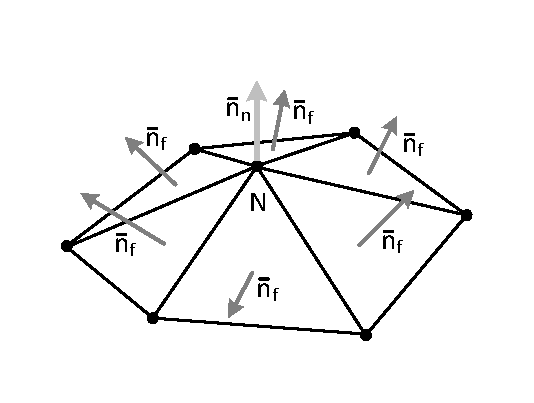
\includegraphics[width=0.48\textwidth]{pics/pic_architecture_size.pdf}
\captionstyle{center}\caption{The architecture of the computational mesh.}\label{fig:pic_architecture}
\end{figure}

%К расчетной сетке предъявляются следующие требования.
The following requirements are imposed on the computational mesh.
%Во-первых, сетка должна быть целостной, то есть каждое ребро имеет ровно два инцидентных узла, отсутствуют изолированные и висячие узлы, а также изолированные ребра.
First, the mesh must be complete, that is, each edge has exactly two incident nodes, there are no isolated and dangling nodes, and no isolated edges.
%Во-вторых, все ячейки должны представлять собой треугольники (это гарантирует, что ячейка является плоской, так как четыре и более произвольных узлов могут не лежать в одной плоскости).
Second, all faces must be triangles (this ensures that the face is flat, since four or more arbitrary nodes may not lie in the same plane).
%И в-третьих, рассматриваются только замкнутые сетки, представляющие собой поверхности, то есть каждое ребро имеет ровно две инцидентные ячейки.
And thirdly, only closed meshes are considered, which are surfaces, that is, each edge has exactly two incident faces (there are no border edges).

\begin{equation}\label{eq_arch}
\begin{cases}
\forall N \Rightarrow \mathscr{E}(N) > 2, \mathscr{F}(N) > 2 \\
\forall e \Rightarrow \mathscr{N}(e) = 2 , \mathscr{F}(e) = 2 \\
\forall f \Rightarrow \mathscr{N}(f) = 3 , \mathscr{E}(f) = 3 \\
\end{cases}
\end{equation}

%В качестве дополнения также будем требовать, чтобы сетка представляла собой двустороннюю поверхность, для каждой ячейки однозначно определена нормаль к поверхности $\vec{n}_f$.
As a supplement, we will also require that the mesh is a two-sided surface, for each face the normal to the surface $\vec{n}_f$ is uniquely defined.
%Также никакие два узла сетки не совпадают и отсутствуют ячейки с нулевой площадью (так как это сделает невозможным вычислений нормалей).
Also, no two mesh nodes are the same and there are no faces with zero area (since this would make it impossible to calculate normals).
%Для узла сетки будем рассматривать понятие нормали к поверхности и определять эту нормаль как
For a mesh node, we will consider the concept of a normal to the surface and define this normal as

\begin{equation}
\vec{n}_n(N) = \frac{1}{|\mathscr{F}(N)|} \sum_{f \in \mathscr{F}(N)}{\vec{n}_f(f)}
\end{equation}

%---------------------------------------------------------------------------------------------------

\section{Remeshing}

%Центральная задача перестроения поверхности из-за нарастания ледяного покрова выглядит следующим образом.
The central task of rebuilding the surface due to the growth of the ice cover is as follows.
%Пусть известно, что в результате численного решения задачи ледообразования конечно-объемным методом \cite{Beaugendre} в каждой ячейке сетки была вычислена масса накопленного льда ($m$).
Let it be known that as a result of the numerical solution of the problem of ice formation by the finite volume method \cite{Beaugendre}, the mass of accumulated ice ($m$) was calculated in each face of the mesh.
%Будем считать плотность льда постоянной, то есть в каждой ячейке также известен объем накопленного льда ($V$).
We will assume that the density of ice is constant, that is, the volume of accumulated ice ($V$) is also known in each face.
%Для каждого узла сетки $N$ требуется найти его новое положение в пространстве $N'$, чтобы для каждой ячейки с узлами $ABC$ объем пространства, ограниченный фигурой $ABCA'B'C'$ соответствовал объему льда, накопленному в данной ячейке.
For each mesh node $N$, it is required to find its new position $N'$ in space so that for each face with nodes $A$, $B$, $C$ the volume of space bounded by the figure $ABCA'B'C'$ corresponds to the volume of ice accumulated in this face.

%Следует отметить, что поставленная задача может не иметь точного решения, и в этом случае следует стремиться к минимизации ошибки по объему (когда фактически образовавшийся объем льда не слишком сильно отличается от целевого объема, то есть разница $V_{ABCA'B'C'} - V$ мала).
It should be noted that the problem posed may not have an exact solution, in which case we should strive to minimize the volume error (when the actually formed volume of ice does not differ too much from the target volume, that is, the difference $V_{ABCA'B'C'} - V$ is relatively small).

%Задачу определения новых положений узлов расчетной сетки можно разделить на две задачи: определение направлений смещения узлов и определение величин смещения.
The task of determining the new positions of the nodes of the computational mesh can be divided into two tasks: determining the directions of displacement of the nodes and determining the displacement values.
%Далее рассмотрим отдельные методы перестроения поверхностей более подробно.
Next, we consider individual methods for rebuilding surfaces in more detail.

\subsection{Classical remeshing methods}

%Простейшие классические методы перестроения выполняются в предположении, что направление смещения узла совпадает с нормалью, проведенной из этого узла.
The simplest classical rebuilding methods are performed under the assumption that the direction of displacement of a node coincides with the normal drawn from this node.
%Таким образом, необходимо лишь определить величину смещения.
Thus, it is only necessary to determine the magnitude of the offset.
%Отметим, что в двумерной постановке можно найти оптимальное решение (обеспечивающее минимальное отклонение по объему от целевого значения) поставленной задачи \cite{Rybakov_2D}.
Note that in the two-dimensional formulation, we can find the optimal solution (providing the minimum deviation in volume from the target value) of the problem posed \cite{Rybakov_2D}.

\begin{figure}[h]
  \centering
  \begin{minipage}[h]{0.49\textwidth}
    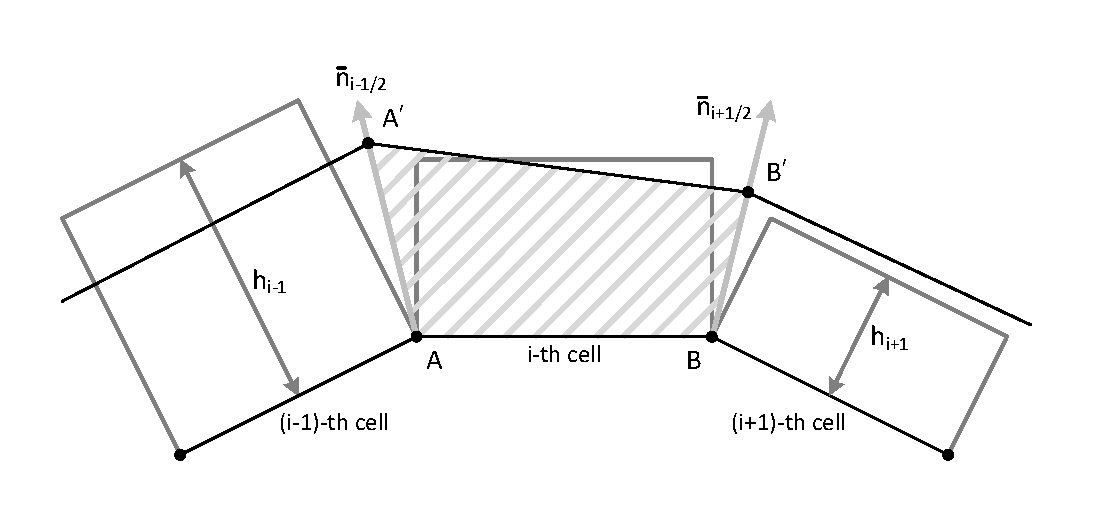
\includegraphics[width=\textwidth]{pics/pic_classical_methods_rectangles_size.pdf}
    \caption{Rebuilding the surface using the method of rectangles in 2D.}\label{fig:pic_classical_methods_rectangles}
  \end{minipage}
  \hfill
  \begin{minipage}[h]{0.49\textwidth}
    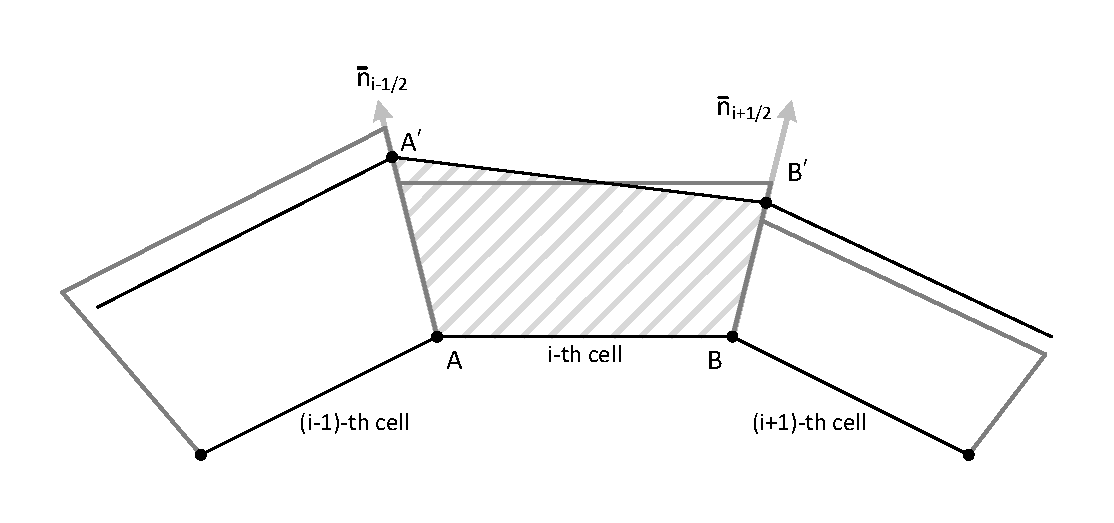
\includegraphics[width=\textwidth]{pics/pic_classical_methods_trapezoids_size.pdf}
    \caption{Surface rebuilding using the trapezoids method in 2D.}\label{fig:pic_classical_methods_trapezoids}
  \end{minipage}
\end{figure}

%В качестве первого метода рассмотрим метод призм (в двумерной постановке аналогом данного метода является метод прямоугольников, продемонстрированный на Fig.~\ref{fig:pic_classical_methods_rectangles}).
As the first method, let's consider the prisms method (in the two-dimensional setting, this method is analogous to the method of rectangles, shown in Fig.~\ref{fig:pic_classical_methods_rectangles}).
%В этом методе входными данными является объем накопленного льда в каждой ячейке сетки ($V(f)$).
In this method, the input data is the amount of accumulated ice in each mesh face ($V(f)$).
%На первым шаге в каждой ячейке ищется толщина ледяного покрова в предположении, что лед в пределах одной ячейки имеет форму призмы, и ячейка является основанием этой призмы.
At the first step, the thickness of the ice cover is searched for in each face, assuming that the ice within one face has the shape of a prism, and the face is the base of this prism.
%Тогда толщина ледяного покрова равняется $h(f) = \frac{V(f)}{S(f)}$, где $S(f)$ -- площадь ячейки.
Then the thickness of the ice cover is equal to $h(f) = \frac{V(f)}{S(f)}$, where $S(f)$ is the face area.
%После чего величина смещения каждого узла вычисляется просто как среднее арифметическое высот ледяного покрова во всех инцидентных ячейках:
After that, the displacement value of each node is calculated simply as the arithmetic average of the ice cover heights in all incident faces:

\begin{equation}
h(N) = \frac{1}{|\mathscr{F}(N)|} \sum_{f \in \mathscr{F}(N)}{h(f)}
\end{equation}

%Второй метод можно назвать методом пирамид (в двумерной постановке аналогом данного метод является метод трапеций, показанный на Fig.~\ref{fig:pic_classical_methods_trapezoids}).
The second method can be called the pyramids method (in a two-dimensional setting, this method is analogous to the trapezoids method shown in Fig.~\ref{fig:pic_classical_methods_trapezoids}).
%Входными данными также является объем накопленного льда в каждой ячейке сетки ($V(f)$).
The input data is also the volume of accumulated ice in each mesh face ($V(f)$).
%Однако в отличие от предыдущего метода объем накопленного в ячейке льда представляется не призмой, а усеченной пирамидой, основанием которой является ячейка, а боковые ребра направлены вдоль нормалей узлов.
However, unlike the previous method, the volume of ice accumulated in the face is represented not by a prism, but by a truncated pyramid, the base of which is the face, and the side edges are directed along the normals of the nodes.
%Высота этой усеченной пирамиды ищется из соотношения $V(f) = \frac{1}{3} h (2S + hS'_h + \sqrt{S(S + hS'_h)})$, где величина $S'_h$ определяется направлениями нормалей узлов ячейки.
The height of this truncated pyramid is found from the relation $V(f) = \frac{1}{3} h (2S + hS'_h + \sqrt{S(S + hS'_h)})$, where $S'_h$ is determined by the directions of the normals of the nodes of the face.
%Тогда как узлы ячейки являются точками первого основания построенной пирамиды, точки второго основания представляют собой новые положения узлов, вычисленных относительно рассматриваемой ячейки.
While the nodes of the face are the points of the first base of the constructed pyramid, the points of the second base are the new positions of the nodes computed relative to the face in question.
%Таким образом, у каждого узла сетки вычисляется несколько новых положений (каждое из которых вычислено относительно своей инцидентной ячейки).
Thus, for each mesh node, several new positions are calculated (each of which is calculated relative to its incident face).
%Для двумерного случая получается ровно два таких новых положения (так как в двумерном случае каждый узел имеет ровно две инцидентные ячейки), для трехмерного случае таких точек более двух.
For the two-dimensional case, exactly two such new positions are obtained (since in the two-dimensional case each node has exactly two incident faces), for the three-dimensional case there are more than two such points.
%Для выбора единственного нового положения узла сетки берется среднее значение из всех положений, вычисленных относительно инцидентных ячеек.
To select a single new mesh node position, the average of all positions computed with respect to the incident faces is taken.

%Из рассмотренных двух методов интуитивно создается впечатление, что метод пирамид должен быть более точным, так как он учитывает потери и избыток объема льда, образующиеся из-за изломов сетки (так как соседние ячейки не лежат в одной плоскости, то представление льда в ячейках в виде призм неизбежно приводит к образованию пробелов или наложений частей льда в виде призм друг на друга).
From the two methods considered, it intuitively gives the impression that the pyramids method should be more accurate, since it takes into account the loss and excess volume of ice formed due to mesh sharp fractures (since neighboring faces do not lie in the same plane, the representation of ice in faces in the form prisms inevitably leads to the formation of gaps or overlapping of ice parts in the form of prisms on top of each other).
%Но по крайней мере в двумерном случае это предположение оказывается неверным, так как метод прямоугольников демонстрирует меньшее отклонение от точного решения по сравнению с методом трапеций \cite{Rybakov_2D}.
But at least in the two-dimensional case, this assumption turns out to be wrong, since the method of rectangles shows a smaller deviation from the exact solution compared to the trapezoids method \cite{Rybakov_2D}.

\begin{figure}[h]
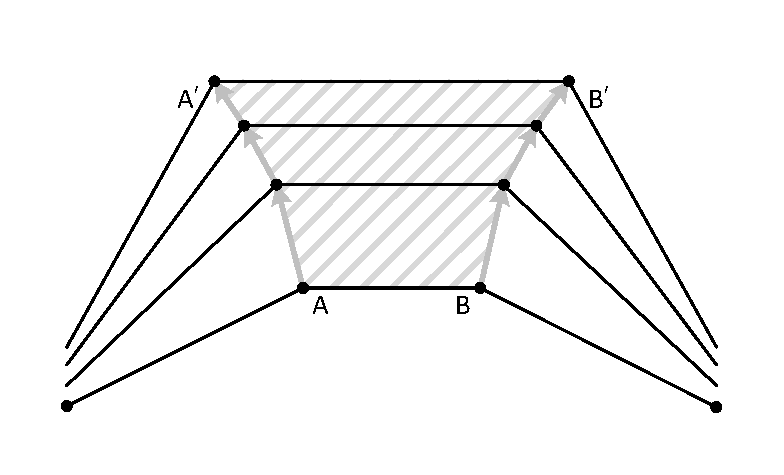
\includegraphics[width=0.48\textwidth]{pics/pic_classical_methods_multilayer_size.pdf}
\captionstyle{center}\caption{Multilayer mesh rebuilding.}\label{fig:pic_classical_methods_multilayer}
\end{figure}

%Вне зависимости от используемого метода перестроения значительно повысить точность можно с помощью многослойного подхода \cite{BourgaultCote}.
Regardless of the rebuilding method used, a significant increase in accuracy can be achieved using a layered \cite{BourgaultCote} approach.
%В этом случае вместо однократного перестроения сетки по объему накопленного льда в каждой ячейке ($V(f)$), выбирается фиксированное количество шагов перестроения $k$, а дальше процедура выполняется $k$ раз подряд, но с использованием объема накопленного в ячейке льда $\frac{V(f)}{k}$.
In this case, instead of a single rebuilding of the mesh by the volume of accumulated ice in each face ($V(f)$), a fixed number of rebuilding steps $k$ is chosen, and then the procedure is performed $k$ times in a row, but using the volume of ice accumulated in the face $\frac{V(f)}{k}$.
%Точность повышается из-за того, что после каждого шага перестроения нормали в узлах сетки меняют свое направление, и общий объем наращиваемого льда становится более криволинейным, лучше учитывает геометрию сетки и, как следствие, точнее соответствует исходному значению $V(f)$ (см. Fig.~\ref{fig:pic_classical_methods_multilayer}).
The accuracy increases due to the fact that after each rebuilding step, the normals at the mesh nodes change their direction, and the total volume of the growing ice becomes more curvilinear, takes into account the mesh geometry better, and, as a result, more accurately corresponds to the initial value of $V(f)$ (Fig.~\ref{fig:pic_classical_methods_multilayer}).

\subsection{Rebuilding with ice volume conservation}

%В работах \cite{Thompson,Tong} описан устойчивый итерационный алгоритм эволюции поверхностной сетки, сохраняющий целевой объем льда.
The articles \cite{Thompson,Tong} describe a stable iterative mesh evolution algorithm that preserves the target volume of ice.
%В нем используется ряд улучшений по сравнению с классическими методами.
It uses several improvements over the classical methods.

%Многослойный подход, реализованный в этом методе, не использует константное количество шагов -- величина наращиваемого объема на каждом шаге алгоритма рассчитывается исходя из максимально допустимой доли временного шага обледенения, после превышения которого возможно развитие численной нестабильности в эволюции поверхности.
The multilayer approach implemented in this method does not use a constant number of steps -- the value of the increased volume at each step of the algorithm is calculated based on the maximum allowable fraction of the icing time step, after exceeding which numerical instability may occur in the evolution of the surface.
%Наиболее очевидный случай возникает, когда проекции нормалей граней пересекаются, в этом случае слишком большой временной шаг приведет к складыванию поверхности.
The most obvious case occurs when the face normal projections intersect, in which case too large a time step will cause the surface to fold.
%Чтобы идентифицировать грани, которые будут демонстрировать подобное поведение на текущем временном шаге, предполагается, что объем, образованный путем вытягивания треугольной грани с использованием параллельной плоскости смещения, образует призматоид, объем которого определяется кубической функцией высоты $h$:
In order to identify faces that will exhibit such behavior at the current time step, it is assumed that the volume formed by extruding a triangular face using a parallel displacement plane forms a prismatoid whose volume is given by the cubic function of the height $h$:

\begin{equation}\label{Tong:1}
V(h)=ah+bh^2+ch^3
\end{equation}

%где константы $a$, $b$, $c$ определяются позициями узлов грани, их нормалей и нормалью грани.
where the constants $a$, $b$, $c$ are determined by the positions of the face nodes, their normals, and the face normal.
%Рассмотрим корни квадратного уравнения, которое получается в результате дифференцирования уравнения \ref{Tong:1}.
Consider the roots of the quadratic equation, which is obtained as a result of differentiation of the equation \ref{Tong:1}.
%Если корни являются положительными вещественными значениями, наименьший положительный корень определяет высоту, на которой достигается максимальный объем, которая обозначается как $V_{max}$, иначе функция монотонна с возрастанием и ограничение на шаг в данной грани не требуется.
If the roots are positive real values, the smallest positive root determines the height at which the maximum volume is reached, which is denoted as $V_{max}$, otherwise the function is monotonic with increasing and no step restriction is required in this face.
%Исходя из этого, можно вычислить максимальную долю временного шага обледенения, которая требуется для обеспечения разумного поведения накопления объема.
From this, it is possible to calculate the maximum fraction of the icing time step that is required to ensure reasonable volume accumulation behavior.
%В дополнение к этому пределу размера шага был введен предел стабильности $\alpha_{jiao}$, который основан на том, как изменяются направления нормалей по мере эволюции поверхности \cite{Jiao}.
In addition to this step size limit, a $\alpha_{jiao}$ stability limit has been introduced, which is based on how normal directions change as the surface evolves \cite{Jiao}.
%Тогда, допустимая доля временного шага для $i$-й грани определяется как
Then, the allowable fraction of the time step for the $i$-th face is defined as

\begin{equation}\label{Tong:2}
\alpha_{\Delta t}^i=
\begin{cases}
min(s_{\Delta t}\frac{V_{max}^i}{V_f},\alpha_{jiao},1), \text{if $V_{max}^i$ exists}, \\
\alpha_{jiao}, \text{if $V_{max}^i$ doesn't exist}
\end{cases}
\end{equation}

%где $s_{\Delta t}$ ($0 < s_{\Delta t} < 1$) -- эмпирически определяемый коэффициент, $V_f$ -- текущий оставшийся объем приращения льда для $i$-й грани.
where $s_{\Delta t}$ ($0 < s_{\Delta t} < 1$) is an empirically determined coefficient, $V_f$ is the current remaining ice increment volume for the $i$-th face.
%Тогда объем, наращенный для текущего шага, равен $\alpha_{\Delta t} V_f$, где $\alpha_{\Delta t}$ представляет собой глобальное минимальное значение для всех граней.
Then the volume built up for the current step is $\alpha_{\Delta t} V_f$, where $\alpha_{\Delta t}$ is the global minimum value for all faces.

%Другой важной особенностью алгоритма является введение первичного и нулевого простанств, описанных в \cite{Jiao_null_space_smooth}.
Another important feature of the algorithm is the introduction of primary and null spaces, described in \cite{Jiao_null_space_smooth}.
%Если эволюционное движение узлов сетки происходит в первичном пространстве, то их перемещение в нулевом пространстве будет сохранять потенциальную точность второго порядка триангуляции поверхности, благодаря чему мы можем  проводить сглаживание поверхности сетки с сохранением объема.
If the evolutionary movement of mesh nodes occurs in primary space, then their movement in zero space will preserve the potential accuracy of the second order of triangulation of the surface, so that we can maintain volume when smoothing the mesh surface.
%В алгоритме используется несколько видов сглаживаний.
The algorithm uses several types of smoothing.

%Первое сглаживание -- сглаживание нормалей в вершинах и ячейках сетки.
The first smoothing is the smoothing of the normals in the mesh nodes and faces.
%Чтобы сделать возможным сглаживание в нулевом пространстве, все нормали в узлах рассчитываются так, чтобы они лежали в первичном пространстве, а перемещение узлов при наращивании льда происходит только по их нормалям.
To make smoothing possible in zero space, all normals at nodes are calculated so that they lie in primary space, and the movement of nodes during ice buildup occurs only along their normals.
%По мере эволюции, на поверхности может усиливаться шум -- если его не контролировать, может возникнуть ситуация, когда двугранный угол между гранями станет слишком малым и ограничит максимальную долю временного шага обледенения.
As evolution progresses, surface noise can increase -- if left unchecked, a situation can arise where the dihedral angle between the faces becomes too small and limits the maximum fraction of the icing time step.
%Для уменьшения поверхностного шума, перед наращиванием льда применяется локальное сглаживание, регулирующее направление смещения узла в проблемных областях, чтобы оно более точно совпадало с направлениями его соседей.
To reduce surface noise, local smoothing is applied before ice builds up, adjusting the direction of node displacement in problem areas so that it more closely matches the directions of its neighbors.
%Этот метод может улучшить гладкость поверхности в некоторых ситуациях.
This method can improve surface smoothness in some situations.
%Основная цель сглаживания нормалей -— вытолкнуть точки из вогнутых областей, где нормали могут локально сходиться.
The main purpose of normal smoothing is to push points out of concave areas where normals can converge locally.
%Сглаживание нормалей достигается с помощью серий взвешенных средних, которые предназначены для придания веса нормалям, генерируемым проблемными областями.
Normal smoothing is achieved using a series of weighted averages, which are designed to give weight to the normals generated by problem areas.

%Второе сглаживание -- сглаживание высот.
The second smoothing is height smoothing.
%После вычисления доли временного шага и объема, наращиваемого для текущего шага, для эволюции поверхности необходимо определить поле высот, которое будет соответствовать этому объему, чтобы по нему определить смещения узлов сетки.
After calculating the fraction of the time step and the volume that is increased for the current step, it is necessary to determine the height field for the evolution of the surface, which will correspond to this volume, in order to determine the offsets of the mesh nodes from it.
%Решение $V(h_i) = \alpha_{\Delta t} V_f$ обеспечивает поле начальных высот, которое используется для движения поверхности.
The solution $V(h_i) = \alpha_{\Delta t} V_f$ provides the initial height field that is used to move the surface.
%Цель дополнительного шага сглаживания высоты состоит в том, чтобы отфильтровать высокочастотный шум в поле высот за счет уменьшения разницы высот между соседними гранями.
The purpose of the additional height smoothing step is to filter out high-frequency noise in the height field by reducing the difference in height between adjacent faces.
%Как правило, высоты двух треугольных граней, имеющих общее ребро, не будут равными.
Usually, the heights of two triangular faces that share a common edge will not be equal.
%На данном шаге используется сглаживание высот с сохранением объема путем его перераспределения между соседними гранями.
At this step, smoothing of heights is used while preserving the volume by redistributing it between adjacent faces.

\begin{figure}
  \centering
  \begin{minipage}[h]{0.49\textwidth}
    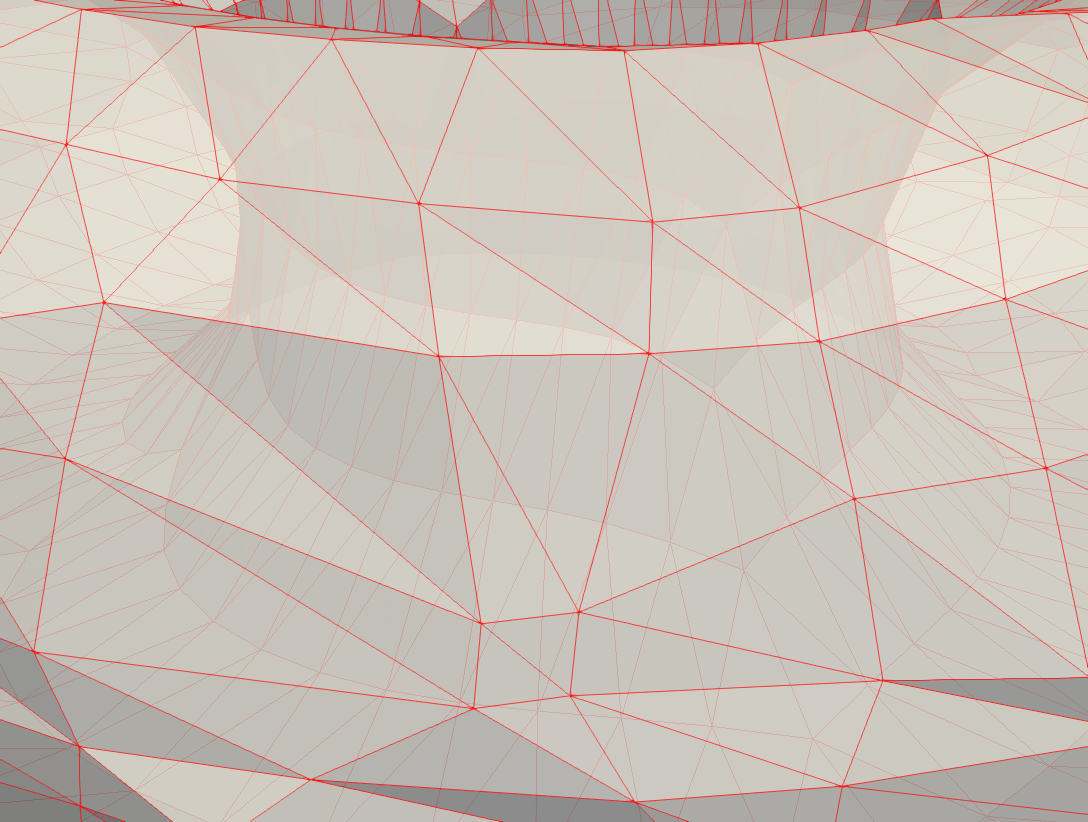
\includegraphics[width=\textwidth]{pics/pic_smooth_before.png}
    \caption{Mesh before null-space smoothing}\label{fig:pic_smooth_before}
  \end{minipage}
  \hfill
  \begin{minipage}[h]{0.49\textwidth}
    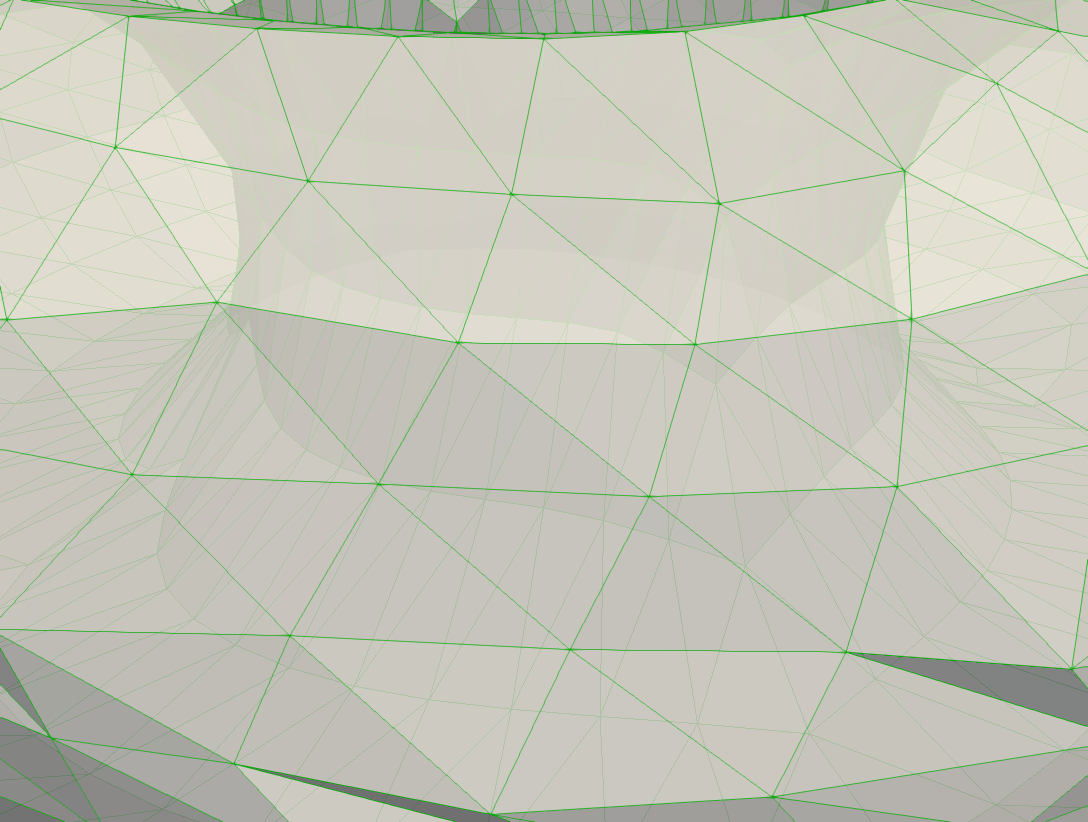
\includegraphics[width=\textwidth]{pics/pic_smooth_after.png}
    \caption{Mesh after null-space smoothing.}\label{fig:pic_smooth_after}
  \end{minipage}
\end{figure}

%Последним типом сглаживания является сглаживание в нулевом пространстве.
The last type of smoothing is null space smoothing.
%Эволюция поверхности будет стремиться упаковать узлы в вогнутые области, где сходятся нормали к поверхности, тогда как расширение сетки происходит в выпуклых областях, где нормали к поверхности расходятся.
Surface evolution will tend to pack nodes into concave regions where surface normals converge, while mesh expansion occurs in convex regions where surface normals diverge.
%Если узлы не будут перераспределены, может стать невозможным продолжать продуктивный, стабильный временной шаг.
If the nodes are not reallocated, it may become impossible to continue with a productive and stable time step.
%Для улучшения качества поверхностной сетки узлы перераспределяются на поверхности с помощью сглаживания в нулевом пространстве.
To improve the quality of the surface mesh, the nodes are redistributed on the surface using null space smoothing.
%Этот метод способен перераспределять точки, сохраняя при этом целостность базовой геометрии.
This method is able to redistribute points while maintaining the integrity of the base geometry.
%Нулевое пространство определяется касательной плоскостью (для гладких областей), касательной линией (для складок поверхности) или пустым пространством (для углов), движущиеся в нем узлы остаются на поверхности, так что объем и форма поверхности могут быть сохранены (Fig.~\ref{fig:pic_smooth_before}, Fig.~\ref{fig:pic_smooth_after}).
Null space is defined by a tangent plane (for smooth areas), a tangent line (for surface wrinkles), or empty space (for corners), nodes moving in it remain on the surface, so that the volume and shape of the surface can be preserved (Fig.~\ref{fig:pic_smooth_before}, Fig.~\ref{fig:pic_smooth_after}).

\subsection{Common envelope method}

%Рассмотрим задачу определения новых положений узлов расчетной сетки немного в другой постановке.
Let us consider the problem of determining the new positions of the nodes of the computational mesh in a slightly different formulation.
%Пусть для каждого узла $\vec{N}$ известна линейная скорость нарастания льда $v(\vec{N})$ (в метрах в секунду).
Let the linear rate of ice growth $v(\vec{N})$ (in meters per second) be known for each node $\vec{N}$.
%Будем считать, что нарастание льда в любой точке роста выполняется одновременно во всех направлениях аналогично принципу Гюйгенса-Френеля распространения волн.
We will assume that the growth of ice at any point of growth is carried out simultaneously in all directions, similar to the Huygens-Fresnel principle of wave propagation.
%Тогда фронт распространения льда от произвольной точки $\vec{P}$ через промежуток времени $\Delta t$ будет иметь форму сферы с центром в точке $\vec{P}$ и радиусом $v(\vec{P}) \Delta t$.
Then the ice propagation front from an arbitrary point $\vec{P}$ after a time interval $\Delta t$ will have the shape of a sphere centered at the point $\vec{P}$ and radius $v(\vec{P}) \Delta t$.
%Далее будем предполагать, что выполняется расчет новых положений узлов через некоторый фиксированный момент времени $\Delta t$, то есть для каждого узла известен радиус продвижения фронта льда $R(\vec{N}) = v(\vec{N}) \Delta t$.
Further, we will assume that the calculation of new positions of the nodes is performed after some fixed time $\Delta t$, that is, for each node, the radius of the ice front advance is known $R(\vec{N}) = v(\vec{N}) \Delta t$.
%Так как элементами расчетной сетки являются треугольники, то необходимо определить радиус продвижения фронта льда для каждой внутренней точки треугольника по данным его вершин.
Since the elements of the computational mesh are triangles, it is necessary to determine the radius of advance of the ice front for each internal point of the triangle according to its vertices.

%Рассмотрим ячейку расчетной сетки, вершинами которой являются точки $\vec{A}$, $\vec{B}$, $\vec{C}$.
Consider a computational mesh face whose vertices are the points $\vec{A}$, $\vec{B}$, $\vec{C}$.
%Точки треугольника представляют собой геометрическое место точек, описываемое следующим образом:
The points of a triangle are the locus of points described as follows:

\begin{equation}
\begin{cases}
\vec{P}(\beta, \gamma) = \vec{A} + \beta (\vec{B} - \vec{A}) + \gamma (\vec{C} - \vec{A}) = \vec{A} + \beta \vec{AB} + \gamma \vec{AC} \\
\beta \ge 0 \\
\gamma \ge 0 \\
\beta + \gamma \le 1
\end{cases}
\end{equation}

%Определим для каждой точки треугольника $\vec{P}(\beta, \gamma)$ радиус продвижения фронта льда как $R(\vec{P}(\beta, \gamma)) = R(\beta, \gamma) = R(\vec{A}) + \beta (R(\vec{B}) - R(\vec{A})) + \gamma (R(\vec{C}) - R(\vec{A})) = R_A + \beta R_{AB} + \gamma R_{AC}$.
Let us define for each point of the triangle $\vec{P}(\beta, \gamma)$ the radius of ice front advance as $R(\vec{P}(\beta, \gamma)) = R(\beta, \gamma) = R(\vec{A}) + \beta (R(\vec{B}) - R(\vec{A})) + \gamma (R(\vec{C}) - R(\vec{A} )) = R_A + \beta R_{AB} + \gamma R_{AC}$.
%Фронт продвижения льда от точки $\vec{P}(\beta, \gamma)$ представляет собой сферу $S(\beta, \gamma) = S(\vec{P}(\beta, \gamma), R(\beta, \gamma))$.
The front of ice advance from the point $\vec{P}(\beta, \gamma)$ is a sphere $S(\beta, \gamma) = S(\vec{P}(\beta, \gamma), R(\beta,\gamma))$.
%Фронтом продвижения льда всей треугольной ячейки будем считать общую огибающую сфер, построенных на всех точках этой ячейки, что показано на Fig.~\ref{fig:pic_general_envelope_size}.
The ice advance front of the entire triangular face is the common envelope of the spheres built on all points of this face, which is shown in Fig.~\ref{fig:pic_general_envelope_size}.

\begin{figure}
  \centering
  \begin{minipage}[b]{0.48\textwidth}
    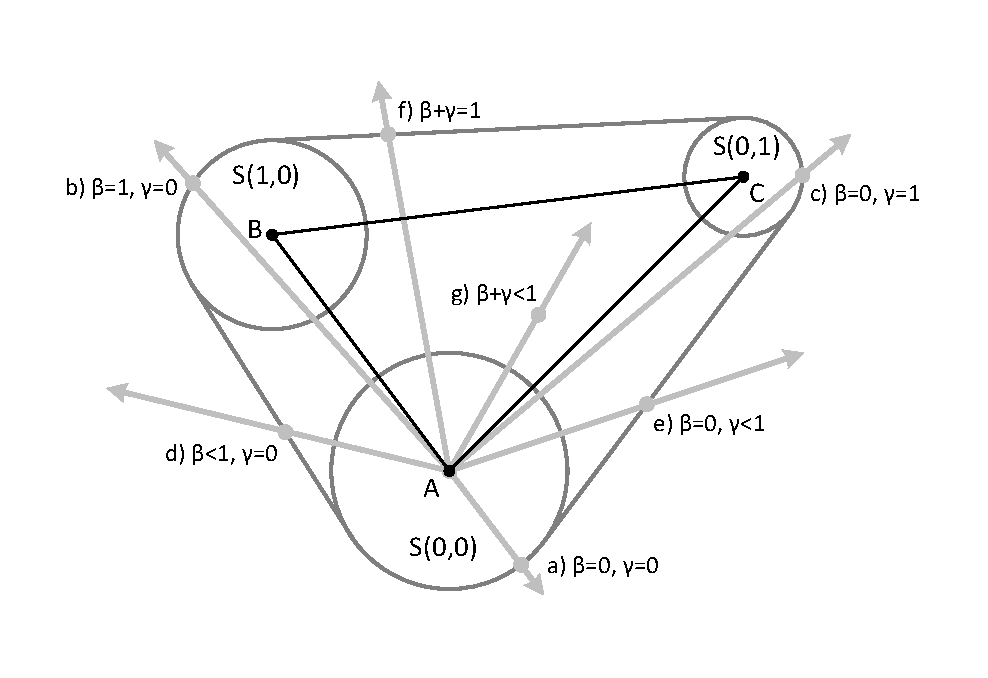
\includegraphics[width=\textwidth]{pics/pic_general_envelope_size.pdf}
    \caption{The common envelope surface of the spheres built on the points of the triangle.}\label{fig:pic_general_envelope_size}
  \end{minipage}
  \hfill
  \begin{minipage}[b]{0.48\textwidth}
    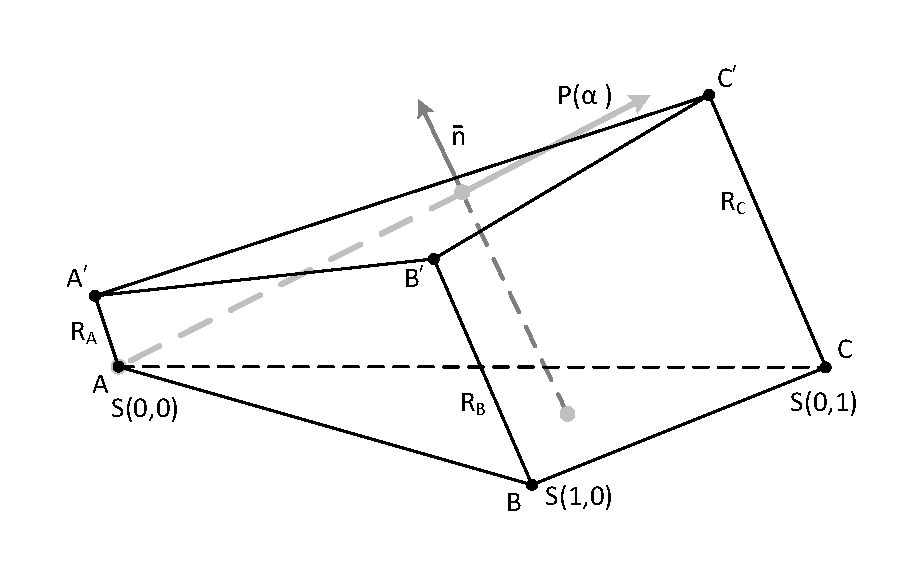
\includegraphics[width=\textwidth]{pics/pic_general_envelope_2_size.pdf}
    \caption{Finding a new node position on the common tangent plane of three spheres.}\label{fig:pic_general_envelope_2_size}
  \end{minipage}
\end{figure}

%При изменении положения узлов расчетной сетки (точки $\vec{A}$, $\vec{B}$, $\vec{C}$) будем исходить из предположения, что после перемещения узлы будут находиться на общей огибающей поверхности множества сфер $S(\beta, \gamma)$ (новые положения узлов -- точки $\vec{A'}$, $\vec{B'}$, $\vec{C'}$).
When changing the position of the nodes of the computational mesh (points $\vec{A}$, $\vec{B}$, $\vec{C}$), we will proceed from the assumption that after moving the nodes will be on the common envelope surface of the set of spheres $ S(\beta, \gamma)$ (new node positions -- points $\vec{A'}$, $\vec{B'}$, $\vec{C'}$).
%Пока в расчете не учитываем влияние соседних расчетных ячеек.
So far, we do not take into account the influence of neighboring computational faces in the calculation.
%Без ограничения общности можно рассмотреть только одну вершину ячейки (точка $\vec{A}$).
Without loss of generality, we can consider only one face vertex (point $\vec{A}$).
%Пусть траектория движения точки $\vec{A}$ описывается уравнением полупрямой $\vec{P}(\alpha) = \vec{A} + \alpha \vec{D}$ при $\alpha \ge 0$.
Let the trajectory of the point $\vec{A}$ be described by the half-line equation $\vec{P}(\alpha) = \vec{A} + \alpha \vec{D}$ for $\alpha \ge 0$.
%$\vec{D}$ -- вектор направления движения точки, можно считать, что $|\vec{D}| = 1$.
$\vec{D}$ is the direction vector of the point, we can assume that $|\vec{D}| = $1.
%Для поиска точек пересечения траектории движения точки $\vec{P}(\alpha) = \vec{A} + \alpha \vec{D}$ с произвольной сферой $S(\beta, \gamma)$ необходимо подставить координаты точки $\vec{P}(\alpha)$ в уравнение сферы $|\vec{P} - \vec{C}(\beta, \gamma)| = R(\beta, \gamma)$, где $\vec{C}(\beta, \gamma)$ -- центр рассматриваемой сферы.
To find the points of intersection of the trajectory of the point $\vec{P}(\alpha) = \vec{A} + \alpha \vec{D}$ with an arbitrary sphere $S(\beta, \gamma)$, it is necessary to substitute the coordinates of the point $ \vec{P}(\alpha)$ into the equation of the sphere $|\vec{P} - \vec{C}(\beta, \gamma)| = R(\beta, \gamma)$, where $\vec{C}(\beta, \gamma)$ is the center of the considered sphere.
%В результате получим следующее уравнение:
As a result, we get the following equation:

\begin{equation}\label{eqn:intersect}
|(\vec{A} + \alpha \vec{D}) - \vec{C}(\beta, \gamma)| = R(\beta, \gamma)
\end{equation}

%Это уравнение нужно решить относительно неизвестной $\alpha$ при фиксированных параметрах $\beta$ и $\gamma$.
This equation must be solved for the unknown $\alpha$ with fixed parameters $\beta$ and $\gamma$.
%Это уравнение является квадратным, оно имеет не более двух корней, которые зависят от параметров $\alpha_{1,2} = \alpha_{1,2}(\beta, \gamma)$.
This equation is quadratic, it has no more than two roots, which depend on the parameters $\alpha_{1,2} = \alpha_{1,2}(\beta, \gamma)$.
%Для определения нового положения точки $\vec{A}$ необходимо найти максимальное значение вещественного корня такого уравнения для всех допустимых значений параметров.
To determine the new position of the point $\vec{A}$, it is necessary to find the maximum value of the real root of such an equation for all admissible values of the parameters.
%При этом точка пересечения траектории движения точки $\vec{A}$ с общей огибающей семейства сфер может находиться на разных участках этой огибающей, что продемонстрировано на Fig.~\ref{fig:pic_general_envelope_size} и связано с условиями, которым удовлетворяют параметры $\beta$ и $\gamma$ (пункты a), b), c) -- пересечение со сферой с центром в вершинах треугольника, пункты d), e), f) -- пересечение со сферой с центром на ребрах треугольника, пункт g) -- пересечение со сферой с центром внутри треугольника).
In this case, the point of intersection of the trajectory of the movement of the point $\vec{A}$ with the common envelope of the family of spheres can be located in different parts of this envelope, which is shown in Fig.~\ref{fig:pic_general_envelope_size} and is associated with the conditions that the parameters $\beta$ and $\gamma$ (points a), b), c) -- intersection with a sphere centered at the vertices of the triangle, points d), e), f) -- intersection with a sphere centered on the edges of the triangle, point g) -- intersection with the sphere centered inside the triangle).

%Уравнение (\ref{eqn:intersect}) можно записать в виде $|\alpha \vec{D} - (\beta \vec{AB} + \gamma \vec{AC})|^2 = (R_A + \beta R_{AB} + \gamma R_{AC})^2$ или в явном виде как квадратное уравнение:
The equation (\ref{eqn:intersect}) can be written as $|\alpha \vec{D} - (\beta \vec{AB} + \gamma \vec{AC})|^2 = (R_A + \beta R_{AB} + \gamma R_{AC})^2$ or explicitly as a quadratic equation:

\begin{equation}
|\vec{D}|^2 \alpha^2 - 2(\beta (\vec{D}, \vec{AB}) + \gamma (\vec{D}, \vec{AC})) \alpha + |\beta \vec{AB} + \gamma \vec{AC}|^2 - (R_A + \beta R_{AB} + \gamma R_{AC})^2 = 0
\end{equation}

%Наибольший корень этого уравнения (с учетом условия $|\vec{D}| = 1$) можно выписать в явном виде:
The largest root of this equation (taking into account the condition $|\vec{D}| = 1$) can be written explicitly:

\begin{multline}
\alpha(\beta, \gamma) = \beta (\vec{D}, \vec{AB}) + \gamma (\vec{D}, \vec{AC}) + \\
\sqrt{(\beta (\vec{D}, \vec{AB}) + \gamma (\vec{D}, \vec{AC}))^2 - |\beta \vec{AB} + \gamma \vec{AC}|^2 + (R_A + \beta R_{AB} + \gamma R_{AC})^2}
\end{multline}

%или
or

\begin{equation}
\begin{cases}
\alpha(\beta, \gamma) = k_{\beta} \beta + k_{\gamma} \gamma + \sqrt{T} \\
T = q_{\beta^2} \beta^2 + q_{\gamma^2} \gamma^2 + q_{\beta \gamma} \beta \gamma + q_{\beta} \beta + q_{\gamma} \gamma + q \\
k_{\beta} = (\vec{D}, \vec{AB}), k_{\gamma} = (\vec{D}, \vec{AC}) \\
q_{\beta^2} = (\vec{D}, \vec{AB})^2 - |\vec{AB}|^2 + R_{AB}^2, q_{\gamma^2} = (\vec{D}, \vec{AC})^2 - |\vec{AC}|^2 + R_{AC}^2 \\
q_{\beta \gamma} = 2 ((\vec{D}, \vec{AB})(\vec{D}, \vec{AC}) - (\vec{AB}, \vec{AC}) + R_{AB} R_{AC}) \\
q_{\beta} = 2 R_A R_{AB}, q_{\gamma} = 2 R_A R_{AC}, q = R_A^2
\end{cases}
\end{equation}

%Для поиска нового положения точки $\vec{A}$ требуется найти максимум выражения $\alpha(\beta, \gamma)$ при условии соблюдения ограничений $\beta \ge 0$, $\gamma \ge 0$, $\beta + \gamma \le 1$.
To search for a new position of the point $\vec{A}$, it is required to find the maximum of the expression $\alpha(\beta, \gamma)$ subject to the constraints $\beta \ge 0$, $\gamma \ge 0$, $\beta + \gamma \le 1$.
%Максимум выражения $\alpha(\beta, \gamma)$ достигается либо при условии нахождения центра сферы внутри треугольника, либо на одной из его сторон.
The maximum of the expression $\alpha(\beta, \gamma)$ is achieved either when the center of the sphere is inside the triangle or on one of its sides.

%В случае нахождения центра сферы на стороне $AB$ треугольника $ABC$ выполняется условие $\gamma = 0$, и выражение для величины $\alpha$ имеет вид $\alpha_{\gamma = 0}(\beta) = k_{\beta} \beta + \sqrt{q_{\beta^2} \beta^2 + q_{\beta} \beta + q}$.
If the center of the sphere is on side $AB$ of triangle $ABC$, the condition $\gamma = 0$ is satisfied, and the expression for $\alpha$ is $\alpha_{\gamma = 0}(\beta) = k_{\ beta} \beta + \sqrt{q_{\beta^2} \beta^2 + q_{\beta} \beta + q}$.
%В случае нахождения центра сферы на стороне $AC$ треугольника $ABC$ выполняется условие $\beta = 0$, и выражение для величины $\alpha$ имеет вид $\alpha_{\beta = 0}(\gamma) = k_{\gamma} \gamma + \sqrt{q_{\gamma^2} \gamma^2 + q_{\gamma} \gamma + q}$.
If the center of the sphere is on side $AC$ of triangle $ABC$, the condition $\beta = 0$ is satisfied, and the expression for $\alpha$ is $\alpha_{\beta = 0}(\gamma) = k_{\ gamma} \gamma + \sqrt{q_{\gamma^2} \gamma^2 + q_{\gamma} \gamma + q}$.
%В случае нахождения центра сферы на стороне $BC$ треугольника $ABC$ выполняется условие $\beta + \gamma = 1$, и выражение для величины $\alpha$ принимает следующий вид:
If the center of the sphere is on side $BC$ of triangle $ABC$, the condition $\beta + \gamma = 1$ is satisfied, and the expression for $\alpha$ takes the following form:

\begin{multline}
\alpha_{\beta + \gamma = 1}(\gamma) = (k_{\gamma} - k_{\beta}) \gamma + k_{\beta} + \\
\sqrt{(q_{\beta^2} + q_{\gamma^2} - q_{\beta \gamma}) \gamma^2 + (-2 q_{\beta^2} + q_{\beta \gamma} - q_{\beta} + q_{\gamma}) \gamma + (q_{\beta^2} + q_{\beta} + q)}
\end{multline}

%Во всех случаях нахождения центра на одной из сторон треугольника задача нахождения максимального значения $\alpha(\beta, \gamma)$ при заданных ограничениях сводится к задаче поиска максимального значения функции вида $\alpha(x) = k_x x + k + \sqrt{q_{x^2} x^2 + q_x x + q}$ (с учетом этих ограничений), что не представляет труда (точкой максимума является либо точка локального экстремума, либо точка границы области определения функции).
In all cases where the center is on one of the sides of the triangle, the problem of finding the maximum value of $\alpha(\beta, \gamma)$ under given constraints is reduced to the problem of finding the maximum value of a function of the form $\alpha(x) = k_x x + k + \sqrt {q_{x^2} x^2 + q_x x + q}$ (taking into account these restrictions), which is not difficult (the maximum point is either a local extremum point or a boundary point of the function's domain).

%Отдельно следует рассмотреть вариант, при котором центр искомой сферы находится внутри треугольника.
Separately, we should consider the option in which the center of the desired sphere is inside the triangle.
%В этом случае точка пересечения траектории $\vec{P}(\alpha) = \vec{A} + \alpha \vec{D}$ с общей огибающей находится на общей касательной плоскости к сферам $S(0, 0)$, $S(1, 0)$, $S(0, 1)$ (плоскость $A'B'C'$, см. Fig.~\ref{fig:pic_general_envelope_2_size}).
In this case, the point of intersection of the trajectory $\vec{P}(\alpha) = \vec{A} + \alpha \vec{D}$ with the common envelope is on the common tangent plane to the spheres $S(0, 0)$, $S(1, 0)$, $S(0, 1)$ (plane $A'B'C'$, see Fig.~\ref{fig:pic_general_envelope_2_size}).

%Центр искомой сферы находится с точке пересечения плоскости $ABC$ и прямой, проходящей через точку $\vec{P}(\alpha)$ и направленной вдоль нормали к плоскости $A'B'C'$.
The center of the desired sphere is found at the point of intersection of the plane $ABC$ and the straight line passing through the point $\vec{P}(\alpha)$ and directed along the normal to the plane $A'B'C'$.
%Если вектор единичной нормали плоскости $A'B'C'$ обозначить через $\vec{n}$, то взаимосвязь точек плоскостей $ABC$ и $A'B'C'$ можно выразить следующим образом:
If the vector of the unit normal of the plane $A'B'C'$ is denoted by $\vec{n}$, then the relationship between the points of the planes $ABC$ and $A'B'C'$ can be expressed as follows:

\begin{equation}
\begin{cases}
\vec{A'} = \vec{A} + \vec{n} R_A \\
\vec{B'} = \vec{B} + \vec{n} R_B \\
\vec{C'} = \vec{C} + \vec{n} R_C
\end{cases}
\end{equation}

%Для нахождения вектора $\vec{n}$ воспользуемся тем фактом, что результат векторного произведения $\vec{A'B'} \times \vec{A'C'}$ коллинеарен вектору $\vec{n}$.
To find the vector $\vec{n}$, we use the fact that the result of the vector product $\vec{A'B'} \times \vec{A'C'}$ is collinear to the vector $\vec{n}$.
%Запишем это в явном виде
Let's write it explicitly

\begin{equation}
(\vec{AB} + \vec{n} R_{AB}) \times (\vec{AC} + \vec{n} R_{AC}) = t \vec{n}
\end{equation}

\begin{equation}
\vec{AB} \times \vec{AC} + R_{AB} (\vec{n} \times \vec{AC}) - R_{AC} (\vec{n} \times \vec{AB}) = t \vec{n}
\end{equation}

\begin{equation}
t
\left[ { \begin{array}{c}
            n_x \\
            n_y \\
            n_z \\
         \end{array} } \right]
+ R_{AC}
\left[ { \begin{array}{c}
            n_y AB_z - n_z AB_y  \\
            n_z AB_x - n_x AB_z \\
            n_x AB_y - n_y AB_x \\
         \end{array} } \right]
- R_{AB}
\left[ { \begin{array}{c}
            n_y AC_z - n_z AC_y \\
            n_z AC_x - n_x AC_z \\
            n_x AC_y - n_y AC_x \\
         \end{array} } \right]
= \vec{AB} \times \vec{AC}
\end{equation}

%Данное соотношение может выполняться при $t > 0$, либо при $t < 0$, что соответствует существованию двух общих касательных плоскостей к трем сферам.
This relation can be satisfied for $t > 0$, or for $t < 0$, which corresponds to the existence of two common tangent planes to three spheres.
%Перепишем приведенное соотношение в виде системы линейных уравнений относительно составляющих нормали при произвольном значении параметра $t$.
Let us rewrite the above relation as a system of linear equations with respect to the components of the normal for an arbitrary value of the parameter $t$.

\begin{equation}
\left[ { \begin{array}{ccc}
             t & R_{AC} AB_z - R_{AB} AC_z & R_{AB} AC_y - R_{AC} AB_y \\
             R_{AB} AC_z - R_{AC} AB_z & t & R_{AC} AB_x - R_{AB} AC_x \\
             R_{AC} AB_y - R_{AB} AC_y & R_{AB} AC_x - R_{AC} AB_x & t \\
         \end{array} } \right]
\left[ { \begin{array}{c}
            n_x \\
            n_y \\
            n_z \\
         \end{array} } \right]
= \vec{AB} \times \vec{AC}
\end{equation}

%Из данной системы уравнений находятся два возможных направления нормали к общей касательной плоскости сфер $S(0,0)$, $S(1,0)$, $S(0, 1)$.
From this system of equations, two possible directions of the normal to the common tangent plane of the spheres $S(0,0)$, $S(1,0)$, $S(0, 1)$ are found.
%Для каждого направления нормали находится плоскость $A'B'C'$ и точка $\vec{P}(\alpha) = \vec{A} + \alpha \vec{D}$ на ней (и сам искомый параметр $\alpha$).
For each direction of the normal, the plane $A'B'C'$ and the point $\vec{P}(\alpha) = \vec{A} + \alpha \vec{D}$ on it (and the required parameter $\ alpha$).
%Данную точку можно учитывать в общем наборе решений только в том случае, если ей соответствует сфера $S(\beta, \gamma)$, параметры которой удовлетворяют трем условиям $\beta \ge 0$, $\gamma \ge 0$, $\beta + \gamma \le 1$.
This point can be taken into account in the general set of solutions only if it corresponds to the sphere $S(\beta, \gamma)$, whose parameters satisfy the three conditions $\beta \ge 0$, $\gamma \ge 0$, $ \beta + \gamma \le 1$.
%Параметры $\beta$ и $\gamma$ можно определить путем поиска точки пересечения прямой $\vec{P}(\alpha) - x \vec{n}$, $x \in \mathbb{R}$ и плоскости $ABC$.
The parameters $\beta$ and $\gamma$ can be determined by finding the intersection point of the line $\vec{P}(\alpha) - x \vec{n}$, $x \in \mathbb{R}$ and the plane $ABC$.

%Таким образом, найдя решения всех потенциально возможных частных случаев, представленных на Fig.~\ref{fig:pic_general_envelope_size}, находим множество решений $\alpha$, из которых для определения актуального нового положения точки $A'$ необходимо взять максимальное.
Thus, having found solutions to all potentially possible special cases presented in Fig.~\ref{fig:pic_general_envelope_size}, we find a set of solutions $\alpha$, from which, to determine the actual new position of the point $A'$, it is necessary to take the maximum one.

%Изложенный выше алгоритм касается определения смещения узла с учетом только одной инцидентной ячейки.
The above algorithm concerns the obtaining of the node offset given only one incident face.
%При рассмотрении отдельного узла сетки требуется вычислить смещение данного узла относительно каждой инцидентной ячейки и выбрать среди этих смещений максимальное.
When considering a separate mesh node, it is required to calculate the displacement of this node relative to each incident face and choose the maximum among these displacements.

\begin{figure}[h]
  \centering
  \begin{minipage}[h]{0.55\textwidth}
    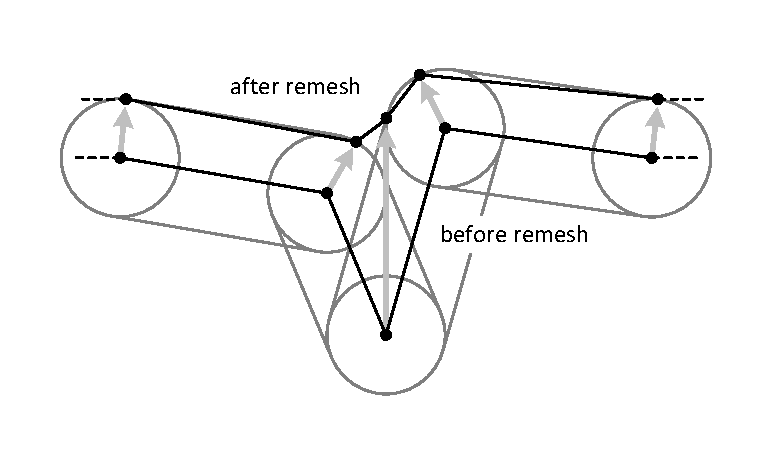
\includegraphics[width=\textwidth]{pics/pic_general_envelope_3_size.pdf}
    \caption{Example of the tightening of a cavity in a 2D diagram.}\label{fig:pic_general_envelope_3_size}
  \end{minipage}
  \hfill
  \begin{minipage}[h]{0.44\textwidth}
    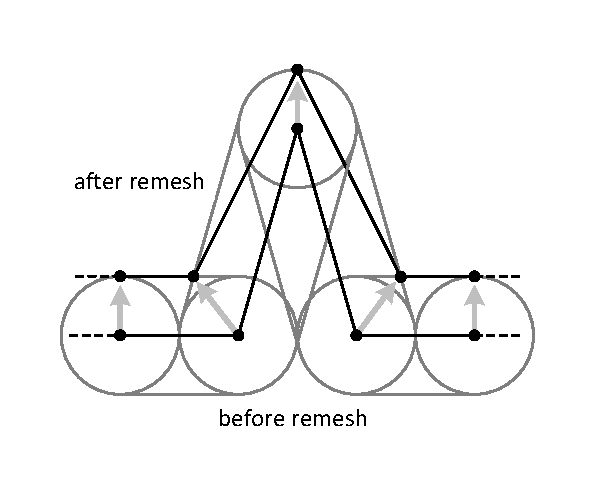
\includegraphics[width=\textwidth]{pics/pic_general_envelope_4_size.pdf}
    \caption{Example of smoothing a sharp peak in a 2D diagram.}\label{fig:pic_general_envelope_4_size}
  \end{minipage}
\end{figure}

\begin{figure}[h]
  \centering
  \begin{minipage}[h]{0.49\textwidth}
    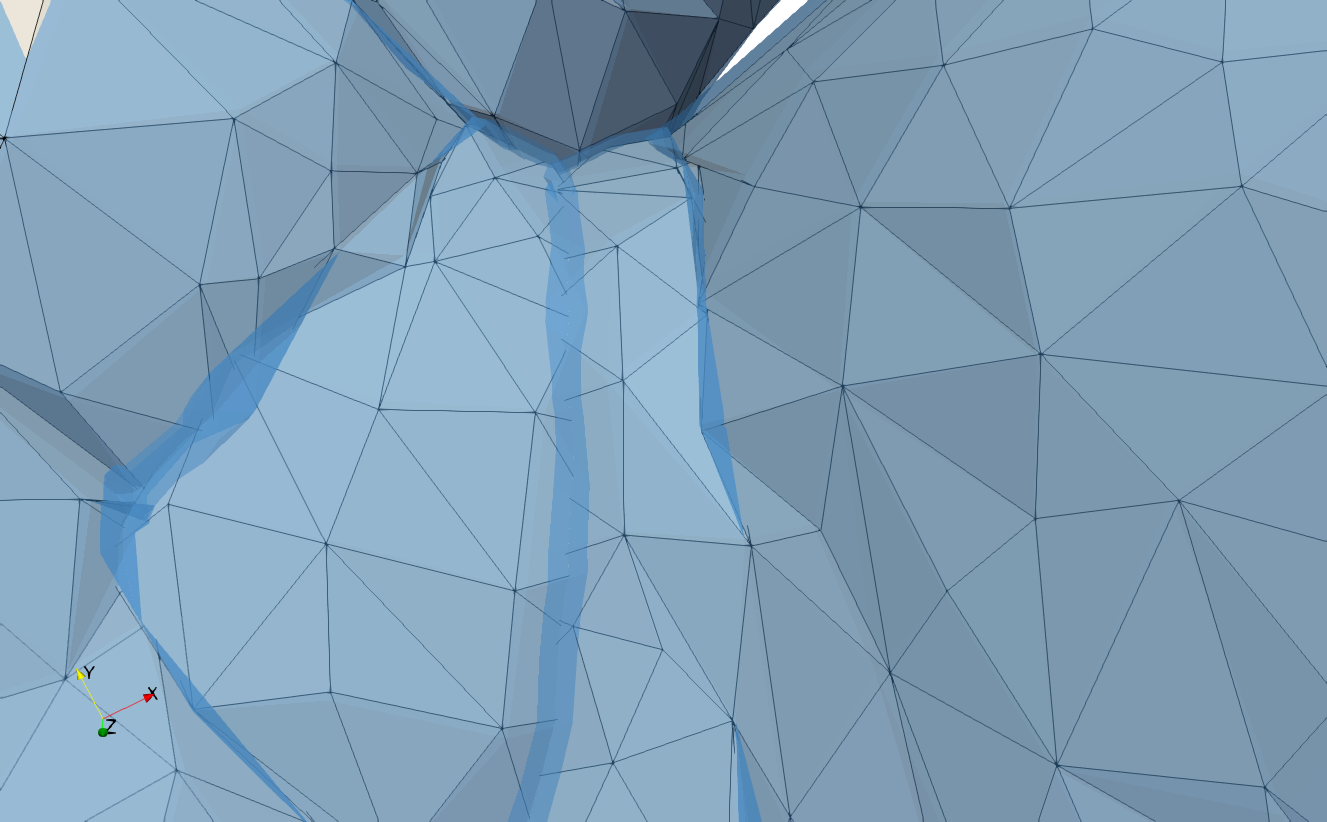
\includegraphics[width=\textwidth]{pics/pic_envelope_cave.png}
    \caption{Example of trough tightening for a 3D surface.}\label{fig:pic_general_envelope_cave}
  \end{minipage}
  \hfill
  \begin{minipage}[h]{0.49\textwidth}
    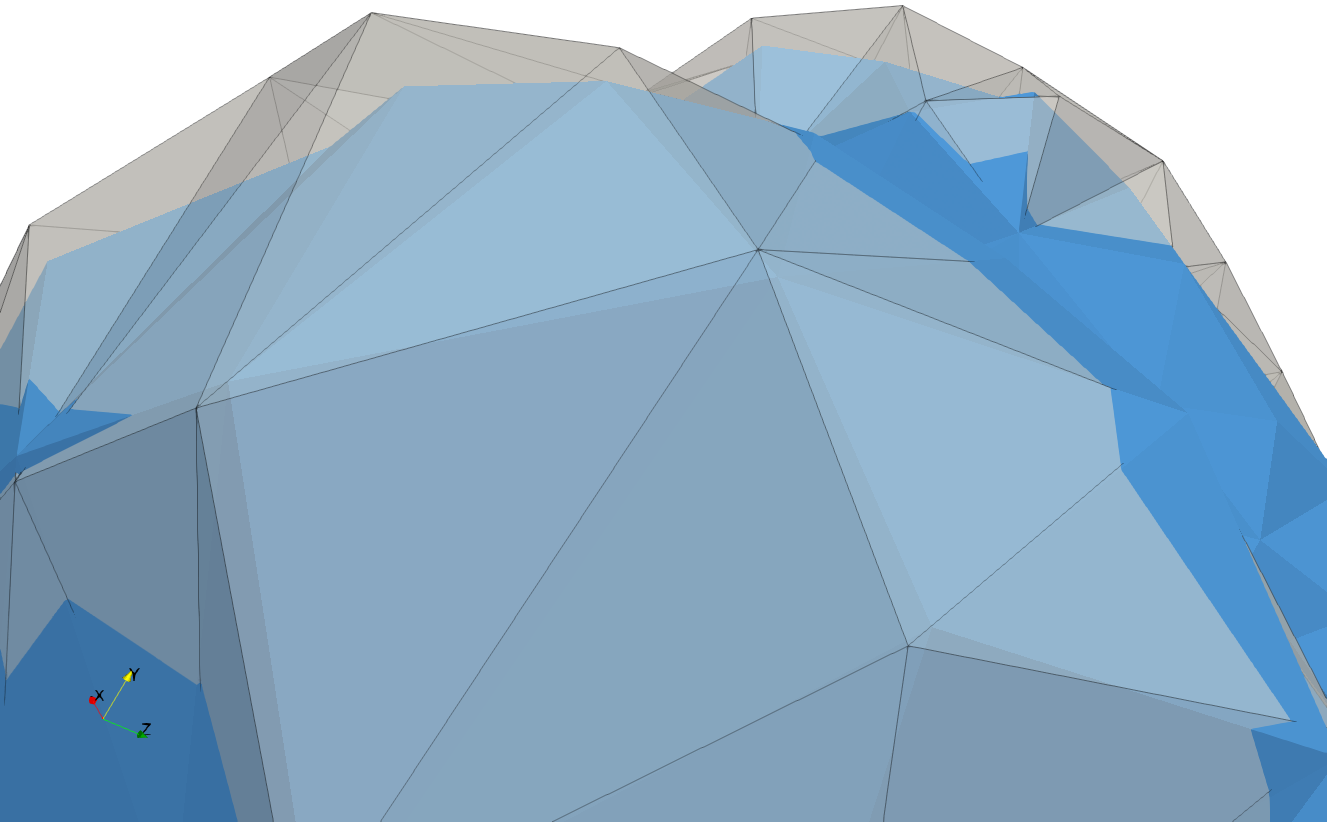
\includegraphics[width=\textwidth]{pics/pic_envelope_peak.png}
    \caption{Example of smoothing sharp peaks for a 3D surface.}\label{fig:pic_envelope_peak}
  \end{minipage}
\end{figure}

%Алгоритм определения новых положений узлов по общей огибающей семейства сфер является линейным по количеству узлов (считаем, что на пригодных к расчетам сетках количество инцидентных ячеек для одного узла ограничено разумным числом) и не содержит итерационных процедур.
The algorithm for determining the new positions of nodes from the common envelope of a family of spheres is linear in the number of nodes (we assume that on meshes suitable for calculations, the number of incident faces for one node is limited by a reasonable number) and does not contain iterative procedures.
%Алгоритм обладает особенностью затягивать мелкие впадины и шумы на сетке.
The algorithm has the peculiarity of tightening small depressions and noise on the mesh.
%Это происходит из-за того, что узел $\vec{N}$, находясь на дне впадины, имеет возможность смещаться по направлению выхода из этой впадины на расстояние, большее $R(\vec{N})$, что продемонстрировано на Fig.~\ref{fig:pic_general_envelope_3_size}.
This is due to the fact that the node $\vec{N}$, being at the bottom of the cavity, has the ability to move in the direction of exit from this cavity to a distance greater than $R(\vec{N})$, which is shown in Fig .~\ref{fig:pic_general_envelope_3_size}.
%Другой интересной особенностью является работа алгоритма на участках сетки с острыми выступами (Fig.~\ref{fig:pic_general_envelope_4_size}).
Another interesting feature is the operation of the algorithm on mesh areas with sharp projections (Fig.~\ref{fig:pic_general_envelope_4_size}).
%Из данного рисунка видно, что в процессе работы алгоритма острые пики имеют тенденцию к сглаживанию.
It can be seen from this figure that during the operation of the algorithm, sharp peaks tend to smooth out.
%Таким образом, новые положения узлов образуют более гладкую поверхность, чем она была до перестроения.
Thus, the new node positions form a smoother surface than it was before the rebuild.

%На Fig.~\ref{fig:pic_general_envelope_cave} продемонстрирован эффект затягивания впадин по сравнению с классическим методом призм (затягивание впадин на сетке отмечено синим цветом).
Fig.~\ref{fig:pic_general_envelope_cave} demonstrates the effect of cavity tightening compared to the classical prisms method (cavity tightening is marked in blue on the mesh).
%На Fig.~\ref{fig:pic_envelope_peak} показан обратный эффект -- сглаживание острых пиков (по сравнению с тем же классическим методом призм).
Fig.~\ref{fig:pic_envelope_peak} shows the opposite effect - smoothing of sharp peaks (compared to the same classical prisms method).

%---------------------------------------------------------------------------------------------------

\section{Adaptation}

%Все рассмотренные в предыдущем разделе методы перестроения поверхностей объединяет одно сходство -- они сохраняют количество элементов расчетной сетки (узлы, ребра, грани) и связи между ними.
All methods of rebuilding surfaces considered in the previous section have one thing in common -- they preserve the number of elements of the computational mesh (nodes, edges, faces) and the connections between them.
%Несмотря на некоторые специальные методы по предотвращению конфликтов между гранями сетки и методы сглаживания, после формирования новой поверхности возможно возникновение самопересечений, появление граней неправильной формы, а также неравномерное распределение граней в сетке по размеру.
Despite some special methods for preventing collisions between mesh faces and smoothing methods, after the formation of a new surface, self-intersections, irregularly shaped faces, and uneven distribution of faces in the mesh in size can occur.
%Пока опустим самопересечения сетки и будем рассматривать только вопросы, касающиеся формы и размера ячеек.
For the time being, we will omit the self-intersections of the mesh and consider only questions concerning the shape and size of the faces.

\begin{figure}[h]
  \centering
  \begin{minipage}[h]{0.35\textwidth}
    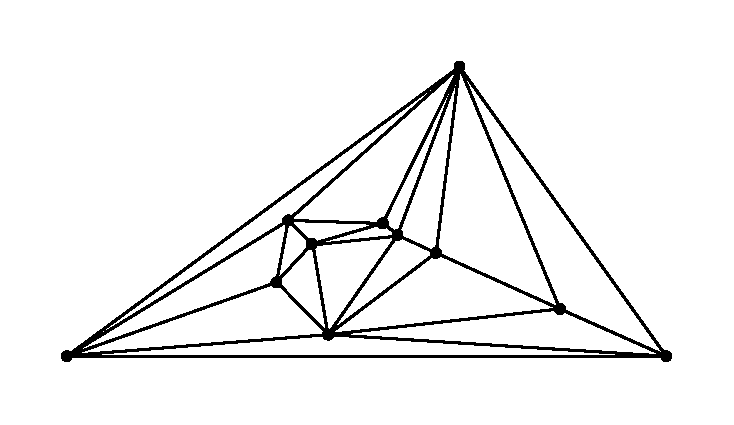
\includegraphics[width=\textwidth]{pics/pic_delaunay_size.pdf}
    \caption{Splitting a face using Delaunay triangulation.}\label{fig:pic_delaunay}
  \end{minipage}
  \hfill
  \begin{minipage}[h]{0.35\textwidth}
    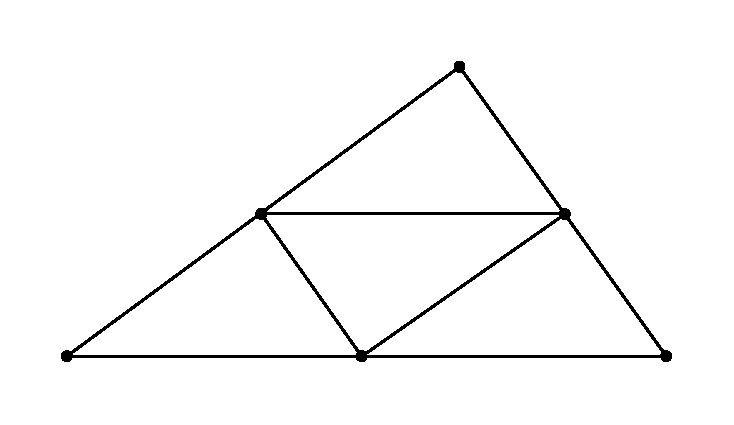
\includegraphics[width=\textwidth]{pics/pic_delaunay_2_size.pdf}
    \caption{Breaking up a face into smaller ones.}\label{fig:pic_delaunay_2}
  \end{minipage}
  \hfill
  \begin{minipage}[h]{0.28\textwidth}
    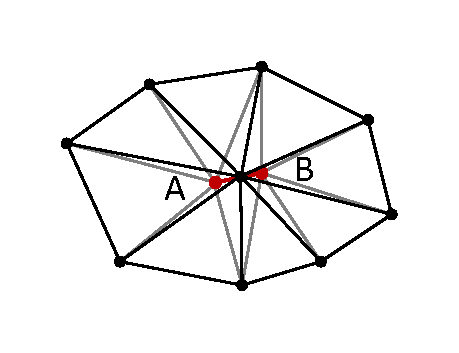
\includegraphics[width=\textwidth]{pics/pic_reduce_edge_size.pdf}
    \caption{Edge reducing.}\label{fig:pic_reduce_edge}
  \end{minipage}
\end{figure}

%Первая операция, которая нам потребуется -- разбиение ячейки на более мелкие.
The first operation that we need is to split the face into smaller ones.
%Во всех случаях будем выполнять разбиение ячеек с помощью триангуляции Делоне, считая что для разбиения нам известен набор точек внутри разбиваемой ячейки (Fig.~\ref{fig:pic_delaunay}) \cite{Rivara}.
In all cases, we will split the faces using Delaunay triangulation, assuming that for splitting we know a set of points inside the split face (Fig.~\ref{fig:pic_delaunay}) \cite{Rivara}.
%Стоит отметить, что разбиение ячейки можно производить с сохранением локальной кривизны сетки, как это показано в \cite{Rakotoarivelo}, но для простоты будем производить разбиение исключительно в плоскости ячейки.
It is worth noting that face partitioning can be performed while preserving the local curvature of the mesh, as shown in \cite{Rakotoarivelo}, but for simplicity, we will partition only in the face plane.
%Если точка разбиения находится не внутри ячейки, а на ее ребре, то разбить придется также вторую инцидентную ячейку этого ребра (рассматриваются только сетки, ребра которых имеют ровно по две инцидентные ячейки, как это указано в (\ref{eq_arch}).
If the split point is located not inside the face, but on its edge, then the second incident face of this edge will also have to be split (only meshes are considered whose edges have exactly two incident faces, as indicated in (\ref{eq_arch}).
%Иногда для уменьшения размера требуется просто разбить ячейку на более мелкие без задания точек разбиения.
Sometimes, to reduce the size, you simply need to split the face into smaller ones without setting split points.
%В этом случае необходимо следить за качеством результирующих ячеек.
In this case, it is necessary to monitor the quality of the resulting faces.
%Для определения качества формы ячейки треугольной формы с узлами $\vec{A}$, $\vec{B}$, $\vec{C}$ можно пользоваться простым критерием качества
To determine the shape quality of a triangular face with nodes $\vec{A}$, $\vec{B}$, $\vec{C}$, we can use a simple quality criterion

\begin{equation}
Q(f) = \frac{4\sqrt{3} S_{ABC}}{|\vec{AB}|^2 + |\vec{BC}|^2 + |\vec{AC}|^2}
\end{equation}

%где $Q(f) = 1$ соответствует идеальному случаю равносторонней ячейки, а $Q(f) = 0$ -- худший случай для ячеек с нулевой площадью \cite{Borouchaki}.
where $Q(f) = 1$ corresponds to the ideal case of an equilateral face, and $Q(f) = 0$ is the worst case for faces with zero area \cite{Borouchaki}.
%Для выполнения разбиения ячейки на более мелкие с сохранением их качества просто выполним разбиение по серединам всех ее сторон (Fig.~\ref{fig:pic_delaunay_2}).
To split a face into smaller ones while maintaining their quality, simply perform a split in the middle of all its sides (Fig.~\ref{fig:pic_delaunay_2}).

%Вторая операция, которая необходима для адаптации сетки, связана с огрублением.
The second operation, which is necessary for mesh adaptation, is related to coarsening.
%Достаточно часто во время выполнения триангуляции по множеству заданных точек могут появляться ячейки с низким показателем качества (у них могут присутствовать либо слишком острые углы, либо близкий к развернутому угол).
Quite often, when performing triangulation over a set of given points, faces with a low quality indicator may appear (they may have either too sharp corners or a corner close to $2 \pi$).
%Если в ячейке присутствует угол, близкий к развернутому, то избавиться от него поможет разбиение по наибольшей стороне (при этом в качестве точки разбиения следует выбрать основание высоты, опущенной из противолежащего узла).
If the face contains an angle close to $2 \pi$, then splitting along the largest side will help to get rid of it (in this case, the base of the height lowered from the opposite node should be chosen as the splitting point).
%Если же в треугольнике присутствуют лишь близкие к острым углы, то значит в нем есть слишком короткая сторона, которая может быть удалена.
If the triangle contains only close to acute angles, then it has a side that is too short, which can be removed.
%При удалении ребра $AB$ удаляются обе инцидентные ей грани, узлы $A$ и $B$ соединяются в единый узел $A'$, а все ребра из множества $\mathscr{E}(A) \cup \mathscr{E}(B)$ перенаправляются на узел $A'$ с учетом удаления повторных (Fig.~\ref{fig:pic_reduce_edge}).
When an edge $AB$ is removed, both faces incident to it are removed, nodes $A$ and $B$ are connected into a single node $A'$, and all edges from the set $\mathscr{E}(A) \cup \mathscr{E} (B)$ are redirected to node $A'$, taking into account the removal of repeats (Fig.~\ref{fig:pic_reduce_edge}).
%Данную операцию будем называть стягиванием ребра \cite{Panchal}.
This operation will be called edge reducing \cite{Panchal}.
%Путем применения стягивания наиболее коротких ребер в расчетной сетке можно добиться произвольной степени огрубления.
By applying the reducing of the shortest edges in the computational mesh, we can achieve an arbitrary degree of coarsening.

%---------------------------------------------------------------------------------------------------

\section{Self-intersections elimination}

%Основной проблемой, с которой можно потенциально столкнуться при эволюции расчетной сетки, является возникновение самопересечений.
The main problem that can potentially be encountered in the evolution of the computational mesh is the occurrence of self-intersections.
%Самопересечение является критическим дефектом сетки, при котором невозможно производить дальнейшие вычисления по моделированию ледообразования, поэтому самопересечения необходимо удалять.
Self-intersection is a critical mesh defect, which makes it impossible to perform further calculations on ice formation modeling, so self-intersections must be removed.
%Во-первых, необходимо определить, какое отношение двух ячеек сетки можно трактовать как самопересечение.
First, it is necessary to determine what ratio of two mesh faces can be interpreted as self-intersection.
%Конечно, простое наличие общих точек у двух ячеек не может служить критерием самопересечения, так как у каждой ячейки есть смежные ячейки (то есть две ячейки могут иметь как общую вершину, так и общее ребро).
Of course, the mere presence of common points in two faces cannot serve as a criterion for self-intersection, since each face has adjacent faces (that is, two faces can have both a common vertex and a common edge).
%Так как смежными могут быть только ячейки, имеющие общие инцидентные объекты (общую инцидентную вершину или общее инцидентное ребро), а все отношения инцидентности прописаны в расчетной сетке, то не представляет труда отделить пересечение ячеек по общему инцидентному объекту от самопересечения.
Since only faces that have common incident objects (a common incident vertex or a common incident edge) can be adjacent, and all incidence relations are written in the computational mesh, it is not difficult to separate the intersection of faces by a common incident object from self-intersection.

\subsection{Search for pairs of intersecting triangles}

%В любом случае для идентификации всех фактов самопересечения сетки требуется проанализировать все пары ячеек и проверить пересечение ячеек в паре (то есть проверить пересечение каждой ячейки с каждой).
In any case, to identify all facts of mesh self-intersection, it is required to analyze all pairs of faces and check the intersection of faces in the pair (that is, check the intersection of each face with each).
%Так как прямой перебор всех пар ячеек имеет квадратичную сложность по количеству ячеек в сетке, то его использование на крупных сетках невозможно.
Since direct enumeration of all pairs of faces has quadratic complexity in terms of the number of faces in the mesh, its use on large meshes is impossible.
%В этом случае целесообразно выполнять поиск пар пересекающихся ячеек с помощью представления множества ячеек в виде специальной древовидной структуры, связанной с ограничением геометрических объектов прямоугольными параллелепипедами в пространстве.
In this case, it is advisable to search for pairs of intersecting faces using the representation of a set of faces in the form of a special tree structure associated with the restriction of geometric objects by rectangular parallelepipeds in space.
%Для начала определим понятие контейнера для произвольного множества точек $M$ в пространстве (будем обозначать его через $[M]$): $[M]$ -- это прямоугольный параллелепипед, являющийся декартовым произведением трех сегментов
First, let's define the concept of a container for an arbitrary set of points $M$ in space (we will denote it by $[M]$): $[M]$ is a rectangular parallelepiped that is the Cartesian product of three segments

\begin{equation}
[M] = \left[\min_{P \in M}{P_x}, \max_{P \in M}{P_x}\right]
      \times \left[\min_{P \in M}{P_y}, \max_{P \in M}{P_y}\right]
      \times \left[\min_{P \in M}{P_z}, \max_{P \in M}{P_z}\right]
\end{equation}

%Контейнер можно рассматривать для произвольного множества точек.
The container can be considered for an arbitrary set of points.
%Мы будем его использовать для ячейки расчетной сетки, а также для множества ячеек.
We will use it for a face of the computational mesh, as well as for a set of faces.
%Так как любой треугольник является выпуклой фигурой, то $[ABC] = [\{A, B, C\}]$, то есть для построения контейнера для треугольника достаточно рассмотреть только его вершины.
Since any triangle is a convex figure, then $[ABC] = [\{A, B, C\}]$, that is, to construct a container for a triangle, it is enough to consider only its vertices.
%При поиске пар пересекающихся ячеек будем использовать следующий факт: если два треугольника пересекаются, то пересекаются и их контейнеры: $ABC \cap A'B'C' \ne \emptyset \Rightarrow [ABC] \cap [A'B'C'] \ne \emptyset$.
When searching for pairs of intersecting faces, we will use the following fact: if two triangles intersect, then their containers also intersect: $ABC \cap A'B'C' \ne \emptyset \Rightarrow [ABC] \cap [A'B'C'] \ne\emptyset$.
%А значит если не пересекаются контейнеры двух треугольников, то не пересекаются и сами треугольники: $[ABC] \cap [A'B'C'] = \emptyset \Rightarrow ABC \cap A'B'C' = \emptyset$.
This means that if the containers of two triangles do not intersect, then the triangles themselves do not intersect: $[ABC] \cap [A'B'C'] = \emptyset \Rightarrow ABC \cap A'B'C' = \emptyset$.
%В отличие от анализа пары треугольников на пересечение, проверка на пересечение двух прямоугольных параллелепипедов со сторонами, параллельными координатным осям, не представляет проблем.
Unlike the analysis of a pair of triangles for intersection, checking for the intersection of two rectangular boxes with sides parallel to the coordinate axes is not a problem.
%То есть па первом этапе будем искать такие пары ячеек, чьи контейнеры пересекаются (будем называть их потенциально пересекающимися ячейками).
That is, at the first stage, we will look for such pairs of faces whose containers intersect (we will call them potentially intersecting faces).

\begin{figure}[h]
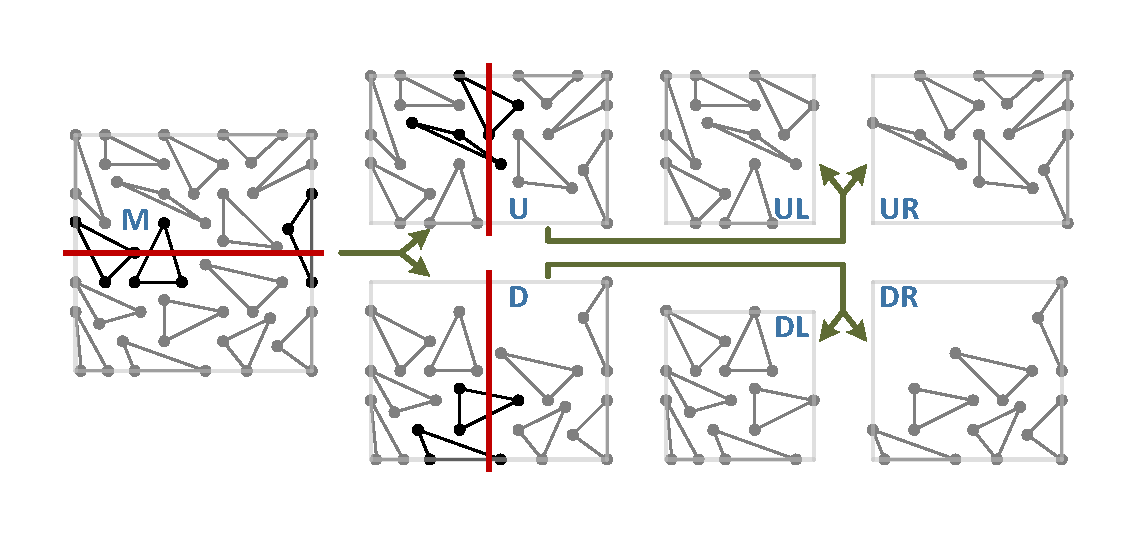
\includegraphics[width=0.8\textwidth]{pics/pic_box_size.pdf}
\captionstyle{center}\caption{Scheme for building a container tree.}\label{fig:pic_box}
\end{figure}

%Для поиска потенциально пересекающихся ячеек построим дерево контейнеров всех ячеек сетки.
To search for potentially intersecting faces, we build a tree of containers for all mesh faces.
%Корнем данного дерева будет являться контейнер всех ячеек расчетной сетки.
The root of this tree will be the container of all faces of the computational mesh.
%Рассмотрим процедуру разделения контейнера на два более мелких на примере двумерного случая, проиллюстрированного на Fig.~\ref{fig:pic_box}.
Consider the procedure for dividing a container into two smaller ones using the two-dimensional case illustrated in Fig.~\ref{fig:pic_box} as an example.
%Путь мы хотим разделить контейнер некоторого множества треугольников ($M$) по горизонтальной прямой на два множества: верхнее ($U$) и нижнее ($D$).
We want to divide the container of some set of triangles ($M$) along a horizontal straight line into two sets: upper set ($U$ -- up) and lower set ($D$ -- down).
%Тогда в верхнее множество попадут все треугольники, лежащие выше прямой, либо пересекающие ее.
Then all triangles that lie above the line or intersect it will fall into the upper set.
%Аналогично в нижнее множество попадут все треугольники, лежащие ниже прямой, либо пересекающие ее.
Similarly, all triangles that lie below the line or intersect it will fall into the lower set.
%После выделения верхнего и нижнего множества треугольников, для каждого из них строятся свои контейнеры, которые становятся дочерними контейнерами исходного.
After selecting the upper and lower sets of triangles, for each of them their own containers are built, which become child containers of the original one.
%После этого получившиеся контейнеры можно делить дальше, используя произвольное направление разбиения ($X$, $Y$, $Z$).
After that, the resulting containers can be divided further using an arbitrary splitting direction ($X$, $Y$, $Z$).
%В частности на Fig.~\ref{fig:pic_box} продемонстрировано разбиение исходного контейнера по схеме $[M] \rightarrow \{[U], [D]\} \rightarrow \{\{[UL], [UR]\}, \{[DL], [DR]\}\}$.
In particular, Fig.~\ref{fig:pic_box} demonstrates the splitting of the original container according to the scheme $[M] \rightarrow \{[U], [D]\} \rightarrow \{\{[UL], [UR]\}, \{[DL], [DR]\}\}$.
%Следует заметить, что за одну операцию контейнер можно разбивать на произвольное количество дочерних контейнеров аналогичным образом.
It should be noted that in one operation, a container can be split into an arbitrary number of child containers in a similar way.
%В качестве же направления разбиения контейнера целесообразно выбирать наиболее протяженное (вдоль которого длина контейнера имеет наибольшее значение).
As the direction of splitting the container, it is advisable to choose the most extended one (along which the length of the container has the greatest value).

%Построенное дерево контейнеров позволяет существенно сократить количество проверяемых потенциальных пересечений треугольников \cite{Jung}, так как если $[M] \cap [M'] = \emptyset$, $[T]$ -- дочерний контейнер для $[M]$, а $[T']$ -- дочерний контейнер для $[M']$, то $[T] \cap [T'] = \emptyset$.
The constructed container tree makes it possible to significantly reduce the number of tested potential intersections of \cite{Jung} triangles, since if $[M] \cap [M'] = \emptyset$, $[T]$ is a child container for $[M]$ , and $[T']$ is a child container for $[M']$, then $[T] \cap [T'] = \emptyset$.

%После того, как найдены все пары потенциально пересекающихся треугольников, необходимо проверить, пересекаются ли они на самом деле.
After all pairs of potentially intersecting triangles have been found, it is necessary to check whether they actually intersect.
%Так как треугольник является выпуклой фигурой, то пересечение двух треугольников также является выпуклой фигурой (это может быть любая плоская фигура с количеством вершин от 1 до 6).
Since a triangle is a convex figure, the intersection of two triangles is also a convex figure (it can be any flat figure with 1 to 6 vertices).
%Вершинами пересечения двух треугольников являются точки пересечения сторон одного треугольника с другим треугольником и наоборот.
The vertices of the intersection of two triangles are the points of intersection of the sides of one triangle with another triangle and vice versa.
%Таким образом задача поиска пересечения двух треугольников сводится к поиску точек пересечения треугольника и отрезка.
Thus, the task of finding the intersection of two triangles is reduced to finding the intersection points of a triangle and a segment.
%Данная задача может быть решена, с помощью представления треугольника $ABC$ в виде геометрического места точек $\vec{P} = \vec{A} + \beta \vec{AB} + \gamma \vec{AC}$, $\beta \ge 0$, $\gamma \ge 0$, $\beta + \gamma \le 1$, представления отрезка $QR$ в виде геометрического места точек $\vec{P} = \vec{Q} + \phi \vec{QR}$, $0 \le \phi \le 1$ и поиска решения системы уравнений $\vec{A} + \beta \vec{AB} + \gamma \vec{AC} = \vec{Q} + \phi \vec{QR}$ относительно неизвестных $\beta$, $\gamma$, $\phi$ с учетом ограничений \cite{Freylekhman}.
This problem can be solved by representing triangle $ABC$ as a locus of points $\vec{P} = \vec{A} + \beta \vec{AB} + \gamma \vec{AC}$, $\ beta \ge 0$, $\gamma \ge 0$, $\beta + \gamma \le 1$, representations of the segment $QR$ as the locus of points $\vec{P} = \vec{Q} + \phi \vec{QR}$, $0 \le \phi \le 1$ and finding a solution to the system of equations $\vec{A} + \beta \vec{AB} + \gamma \vec{AC} = \vec{Q} + \phi \vec{QR}$ with respect to the unknowns $\beta$, $\gamma$, $\phi$ subject to \cite{Freylekhman} constraints.

\subsection{Fixing intersecting triangles}

%После того, как найдены все пары пересекающихся ячеек и области их пересечения, необходимо определить стратегию их устранения.
After all pairs of intersecting faces and areas of their intersection are found, it is necessary to determine a strategy for their elimination.
%Все ячейки расчетной сетки можно разделить на три категории.
All faces of the computational mesh can be divided into three categories.
%Первая категория -- ячейки, которые не пересекаются ни с какими другими ячейками, и которые должны стать частью итоговой поверхности (будем считать, что в любой момент времени у нас есть возможность указать произвольное количество таких ячеек).
The first category is faces that do not intersect with any other faces, and which should become part of the final surface (we will assume that at any time we have the opportunity to specify an arbitrary number of such faces).
%Будем такие ячейки называть статические.
We will call such faces static.
%Вторая категория -- ячейки, которые не пересекаются ни с какими другими ячейками, но которые не должны стать частью итоговой поверхности (ячейки внутренних петель самопересечения поверхности, которые должны быть удалены).
The second category is faces that do not intersect with any other faces, but that should not become part of the final surface (faces of internal self-intersection loops of the surface that must be removed).
%Такие ячейки будем называть скрытыми.
We will call such faces hidden.
%Третья категория -- ячейки, которые пересекаются с какими-то другими ячейками. 
The third category is faces that intersect with some other faces.
%Такие ячейки будем называть ячейками пересечения.
Such faces will be called intersection faces.

\begin{figure}[h]
  \centering
  \begin{minipage}[h]{0.32\textwidth}
    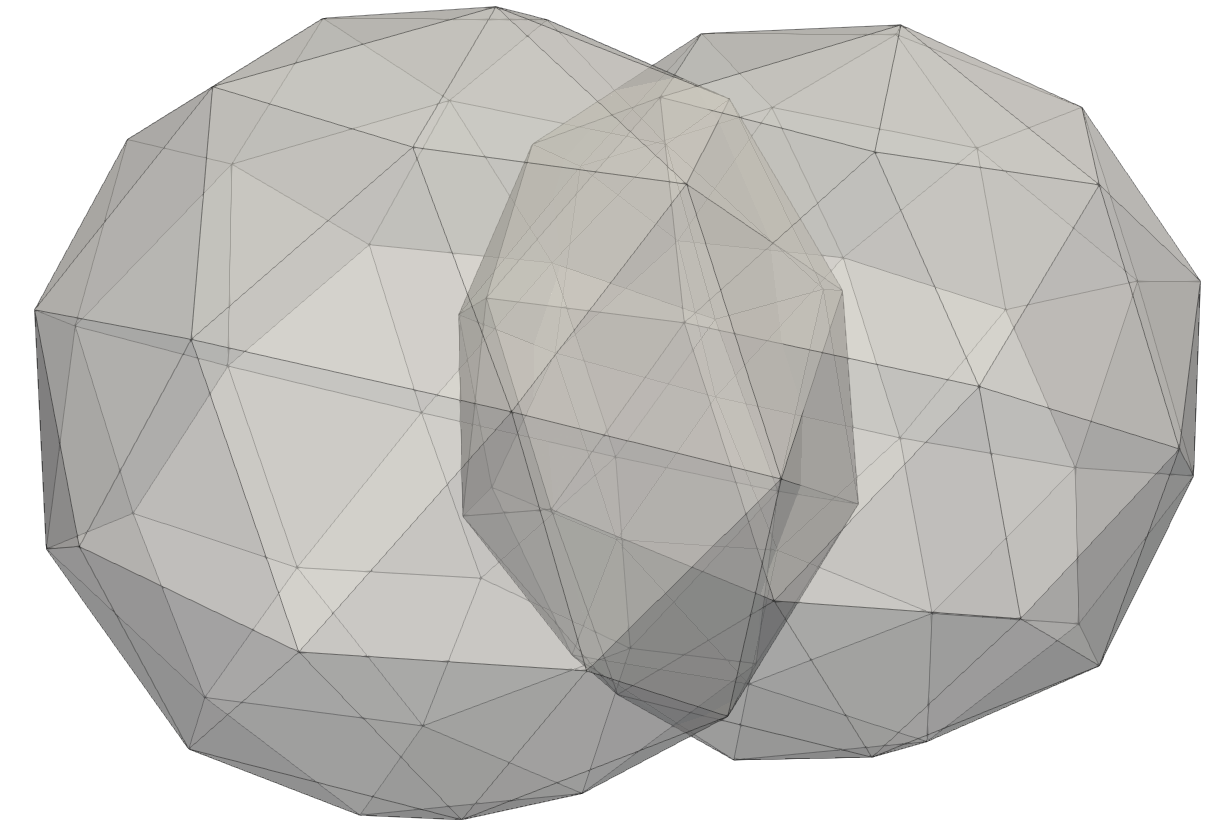
\includegraphics[width=\textwidth]{pics/pic_zip_01.png}
    \caption{Intersection of computational meshes for two spheres.}\label{fig:pic_zip_01}
  \end{minipage}
  \hfill
  \begin{minipage}[h]{0.32\textwidth}
    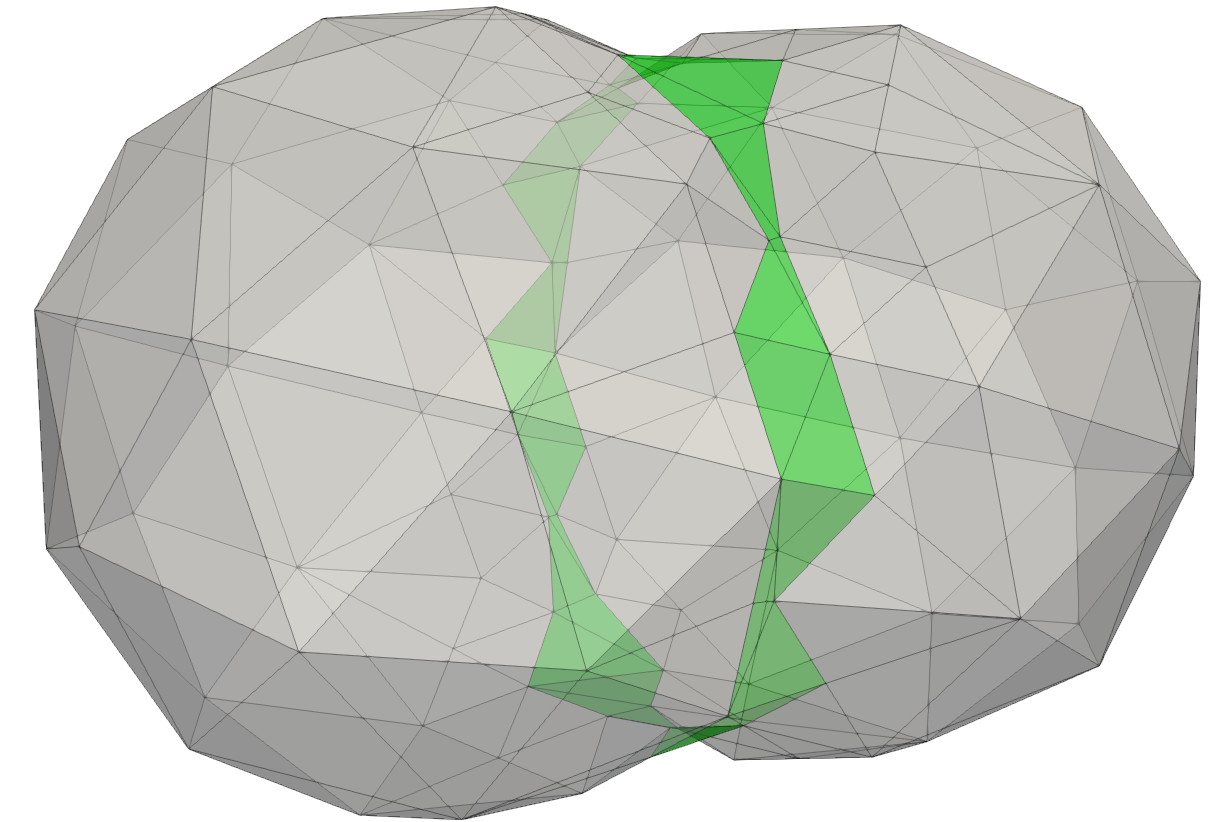
\includegraphics[width=\textwidth]{pics/pic_zip_09.png}
    \caption{Rough removal of intersection faces.}\label{fig:pic_zip_09}
  \end{minipage}
  \hfill
  \begin{minipage}[h]{0.32\textwidth}
    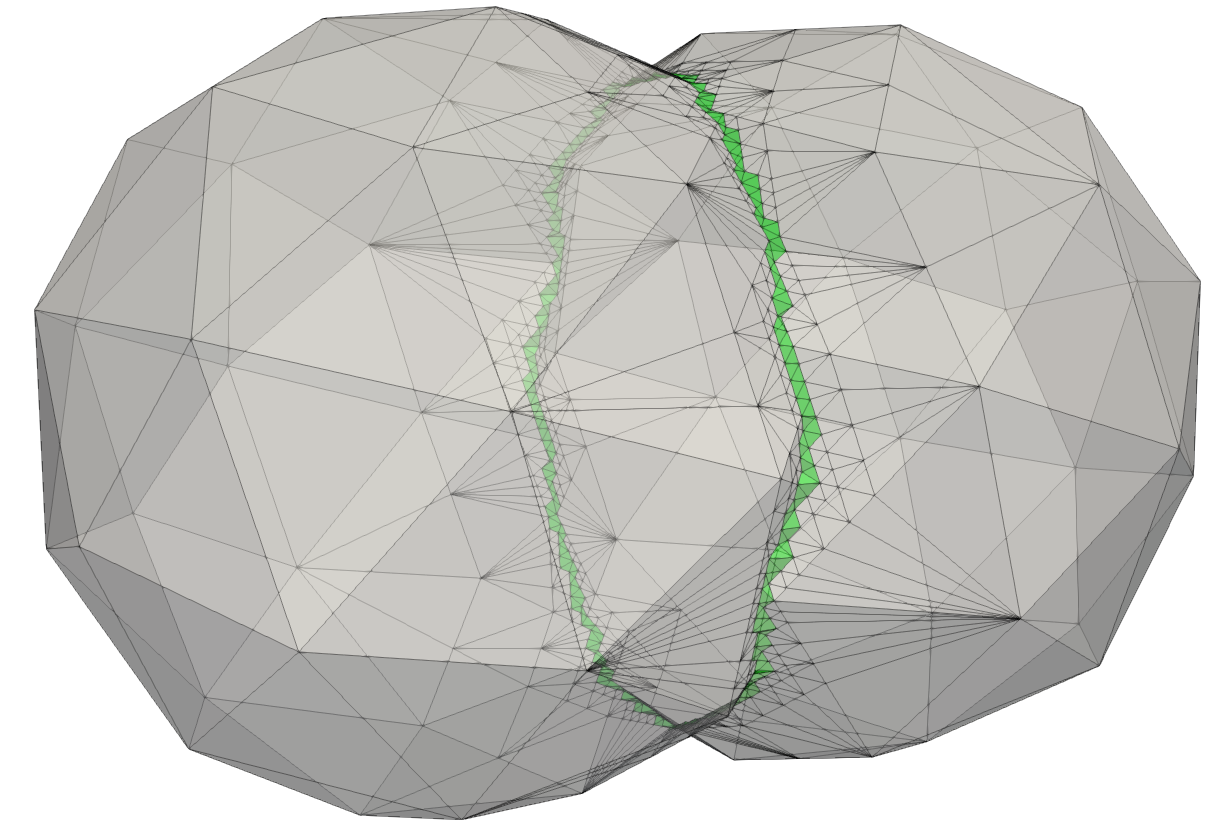
\includegraphics[width=\textwidth]{pics/pic_zip_15.png}
    \caption{Removing intersection faces after splitting.}\label{fig:pic_zip_15}
  \end{minipage}
\end{figure}

%Одним из подходов к устранению самопересечений сетки является просто удаление всех ячеек пересечения.
One approach to eliminating mesh self-intersections is to simply remove all intersection faces.
%После выполнения этой операции сетка распадается на области статических и скрытых ячеек.
After performing this operation, the mesh is divided into areas of static and hidden faces.
%При этом скрытые ячейки являются недостижимыми из статических при выполнении обхода ячеек расчетной сетки (если в процессе обхода соседними считаются только ячейки, смежные по ребру).
In this case, the hidden faces are unreachable from the static ones when the faces of the computational mesh are bypassed (if only the faces adjacent along the edge are considered neighbors during the bypass).
%После удаления из сетки скрытых ячеек расчетная сетка состоит только из статических ячеек, однако требуется добавление новых ячеек для восстановления целостности сетки \cite{Charton}.
After the hidden faces are removed from the mesh, the computational mesh consists only of static faces, but new faces must be added to restore the integrity of the mesh \cite{Charton}.
%Такой подход к устранению самопересечений сетки может применяться для сравнительно простых поверхностей, но в общем случае он не гарантирует получение корректного результата.
This approach to eliminating mesh self-intersections can be used for relatively simple surfaces, but in general it does not guarantee a correct result.
%В качестве иллюстрации такого способа устранения пересечений на Fig.~\ref{fig:pic_zip_01}, Fig.~\ref{fig:pic_zip_09} приведен пример работы для устранения пересечений расчетных сеток двух сфер (новые ячейки, появляющиеся при восстановлении сетки отмечены зеленым цветом).
As an illustration of such a way to eliminate intersections, Fig.~\ref{fig:pic_zip_01}, Fig.~\ref{fig:pic_zip_09} shows an example of work to eliminate intersections of the computational meshes of two spheres (new faces that appear when the mesh is restored are marked in green).
%На Fig.~\ref{fig:pic_zip_09} можно отметить, достаточно низкое качество результирующей сетки.
In Fig.~\ref{fig:pic_zip_09} we can note the rather low quality of the resulting mesh.
%Повысить качество можно с помощью дробления ячеек пересечения.
It is possible to improve the quality by splitting the intersection faces.
%То есть после поиска всех ячеек пересечения, их необходимо раздробить на более мелкие (как показано на Fig.~\ref{fig:pic_delaunay_2}), после чего повторить процедуру удаления ячеек пересечения и скрытых ячеек и выполнить восстановление сетки.
That is, after searching for all intersection faces, they must be split into smaller ones (as shown in Fig.~\ref{fig:pic_delaunay_2}), then repeat the procedure for deleting intersection faces and hidden faces and restore the mesh.
%Процесс дробления ячеек пересечения можно повторять многократно, при этом качество результирующей сетки будет повышаться, как это показано на Fig.~\ref{fig:pic_zip_15}.
The process of splitting the intersection faces can be repeated many times, while the quality of the resulting mesh will increase, as shown in Fig.~\ref{fig:pic_zip_15}.

%При другом подходе устранения самопересечений никакие ячейки из сетки не удаляются, а дробятся на более мелкие по всем точкам пересечения \cite{Skvorkovska}.
With another approach to eliminate self-intersections, no faces are removed from the mesh, but are split into smaller ones at all intersection points \cite{Skvorkovska}.
%В качестве примера на Fig.~\ref{fig:pic_before_cut} показаны два треугольника, которые пересекаются по отрезку (две точки пересечения).
As an example, Fig.~\ref{fig:pic_before_cut} shows two triangles that intersect along a segment (two points of intersection).
%После выполнения дробления получаем конструкцию, показанную на Fig.~\ref{fig:pic_after_cut}.
After crushing, we get the construction shown in Fig.~\ref{fig:pic_after_cut}.
%В общем случае точек, по которым необходимо разбивать ячейку, может быть сколь угодно много, и дробление должно выполняться с помощью выполнения триангуляции по этим точкам, причем некоторые ребра триангуляции должны быть фиксированы.
In the general case, there can be an arbitrarily large number of points at which it is necessary to split a face, and splitting should be performed by triangulating over these points, and some edges of the triangulation should be fixed.

\begin{figure}[h]
  \centering
  \begin{minipage}[h]{0.4\textwidth}
    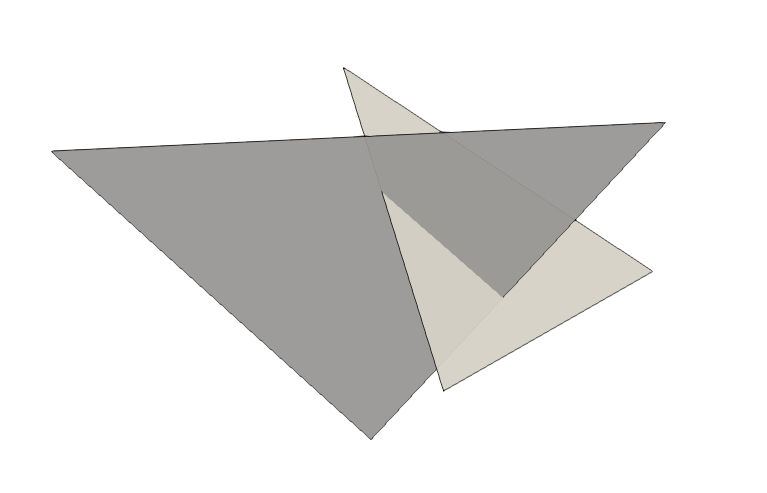
\includegraphics[width=\textwidth]{pics/pic_before_cut.png}
    \caption{Two intersecting triangles before splitting.}\label{fig:pic_before_cut}
  \end{minipage}
  \begin{minipage}[h]{0.4\textwidth}
    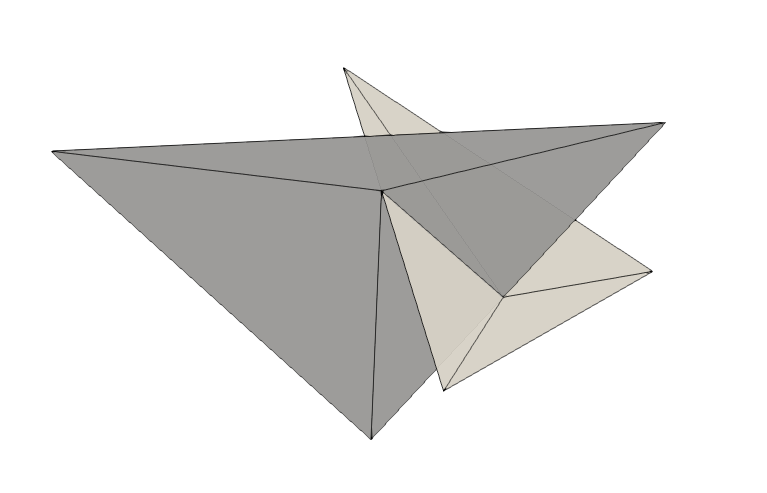
\includegraphics[width=\textwidth]{pics/pic_after_cut.png}
    \caption{Faces after splitting by intersection points.}\label{fig:pic_after_cut}
  \end{minipage}
\end{figure}

%После дробления ячеек по точкам пересечения, между ячейками сетки могут остаться только следующие виды отношений: две ячейки не имеют общих точек, две ячейки имеют одну общую вершину, две ячейки имеют одно общее ребро.
After splitting the faces by intersection points, only the following types of relations can remain between the faces of the mesh: two faces do not have common points, two faces have one common vertex, two faces have one common edge.
%При этом в сетке появляются ребра, имеющие более двух инцидентных ячеек.
In this case, edges appear in the mesh that have more than two incident faces.
%Если наложить на исходную сетку два дополнительных условия, которые могут быть достигнуты с помощью локальных преобразований сетки, то можно добиться достаточно простой структуры сетки (такие сетки будем называть простыми).
If we impose two additional conditions on the original mesh, which can be achieved using local mesh transformations, then we can achieve a fairly simple mesh structure (we will call such meshes simple).
%Первым условием будем считать отсутствие в сетке совпадающих вершин.
The first condition is the absence of matching vertices in the mesh.
%Вторым условием будем считать то, что никакой узел сетки не находится ни в какой другой ячейке.
The second condition is that no mesh node is located in any other face.
%При выполнении этих двух дополнительных условий можно утверждать, что если ребро имеет более двух инцидентных ячеек, то это количество в точности равно 4, причем эти 4 инцидетные ячейки попарно находятся в одной плоскости.
If these two additional conditions are satisfied, we can state that if an edge has more than two incident faces, then this number is exactly 4, and these 4 incident faces are pairwise in the same plane.

\begin{figure}[h]
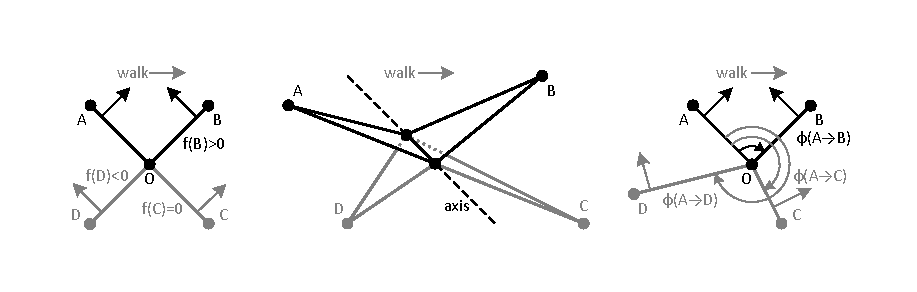
\includegraphics[width=1.0\textwidth]{pics/pic_walk_1_size.pdf}
\captionstyle{center}\caption{Scheme for bypassing the resulting surface.}\label{fig:pic_walk}
\end{figure}

%Для получения результирующей поверхности необходимо избавиться от лишних ячеек, чтобы у каждого ребра вновь осталось ровно по 2 инцидентные ячейки.
To obtain the resulting surface, it is necessary to get rid of extra faces so that each edge again has exactly 2 incident faces.
%Для этого нужно выполнить обход сетки, начиная с любой статической ячейки, считая соседними две ячейки, имеющие общее инцидентное ребро (помечаемые в процессе обхода ячейки попадут в результирующую сетку).
To do this, it is necessary to traverse the mesh, starting from any static face, considering two faces adjacent that have a common incident edge (the faces marked during the traversal will fall into the resulting mesh).
%При движении от некоторой ячейки через ребро, имеющее более двух инцидентных ячеек, возникает вопрос выбора ячейки, которая должна войти в результирующую сетку (при этом все остальные ячейки должны быть удалены).
When moving from a certain face through an edge that has more than two incident faces, the question arises of choosing a face that should enter the resulting mesh (while all other faces should be deleted).

%Рассмотрим процедуру выбора следующей ячейки обхода сетки для ребер, имеющих количество инцидентных ячеек, больше двух (Fig.~\ref{fig:pic_walk}, в центре).
Consider the procedure for selecting the next mesh walk face for edges with more than two incident faces (Fig.~\ref{fig:pic_walk}, center).
%На данном рисунке обозначено направление обхода слева направо, вслед за ячейкой, инцидентной вершине $A$, в результирующую сетку должна войти ячейка, инцидентная вершине $B$.
In this figure, the direction of traversal is indicated from left to right, after the face incident with the vertex $A$, the face incident with the vertex $B$ should enter the resulting mesh.
%Рассмотрим эту процедуру для простых сеток, а также для сеток в общем виде.
Consider this procedure for simple meshes, as well as for meshes in general.
%Для простоты будем рассматривать задачу в проекции на плоскость, перпендикулярную ребру.
For simplicity, we will consider the problem in projection onto a plane perpendicular to the edge.

%Для начала будем считать, что имеет место случай простой сетки (Fig.~\ref{fig:pic_walk}, слева).
To begin with, we will assume that the case of a simple mesh takes place (Fig.~\ref{fig:pic_walk}, left).
%Пусть уже известно, что ячейка, инцидентная вершине $A$, помечена, а ее внешняя нормаль равна $\vec{n}_A$.
Let it be already known that the face incident to the vertex $A$ is labeled and its outward normal equals $\vec{n}_A$.
%Из оставшихся трех ячеек (инцидентных вершинам $B$, $C$, $D$ соответственно) необходимо выбрать только одну для продолжения обхода сетки, а остальные удалить.
Of the remaining three faces (incidental to the vertices $B$, $C$, $D$, respectively), it is necessary to choose only one to continue traversing the mesh, and delete the rest.
%Так как сетка у нас простая, то $\angle AOC = \angle BOD = 2 \pi$, а значит $(\vec{n}_A, \vec{OB}) > 0$, $(\vec{n}_A, \vec{OC}) = 0$, $(\vec{n}_A, \vec{OD}) < 0$.
Since we have a simple mesh, then $\angle AOC = \angle BOD = 2 \pi$, which means $(\vec{n}_A, \vec{OB}) > 0$, $(\vec{n} _A, \vec{OC}) = 0$, $(\vec{n}_A, \vec{OD}) < 0$.
%Таким образом, из всех ячеек, необходимо выбрать ту, для которой значение $(\vec{n}_A, \vec{OP})$ максимально.
Thus, from all faces, it is necessary to choose the one for which the value of $(\vec{n}_A, \vec{OP})$ is maximum.

%Теперь рассмотрим расчетную сетку в общем виде.
Now consider the computational mesh in general case.
%В этом случае количество ячеек, инцидентных рассматриваемому ребру, может быть произвольным, больше двух, а про значение функции $(\vec{n}_A, \vec{OP})$ сказать ничего нельзя.
In this case, the number of faces incident to the considered edge can be arbitrary, more than two, and nothing can be said about the value of the function $(\vec{n}_A, \vec{OP})$.
%Для выбора следующей ячейки для обхода сетки будем поворачивать текущую ячейку вокруг рассматриваемого ребра в направлении $\vec{n}_A$ до совпадения с первой ячейкой (Fig.~\ref{fig:pic_walk}, справа).
To select the next face to bypass the mesh, we will rotate the current face around the considered edge in the direction of $\vec{n}_A$ until it coincides with the first face (Fig.~\ref{fig:pic_walk}, on the right).
%Первая ячейка и должна быть выбрана в качестве следующей для продолжения обхода.
The first face must be selected as the next one to continue the mesh traverse.
%Если через $\phi(A \rightarrow P)$  обозначить угол поворота исходной ячейки в направлении $\vec{n}_A$ до ячеки, инцидентной вершине $P$, то в качестве следующей ячейки для обхода необходимо выбрать ту, для которой $\phi(A \rightarrow B)$ будет минимально.
If we denote by $\phi(A \rightarrow P)$ the angle of rotation of the original face in the direction $\vec{n}_A$ to the face incident with the vertex $P$, then as the next face to be traversed, one must choose the one for which $ \phi(A \rightarrow B)$ will be minimal.

\begin{figure}[h]
  \centering
  \begin{minipage}[h]{0.49\textwidth}
    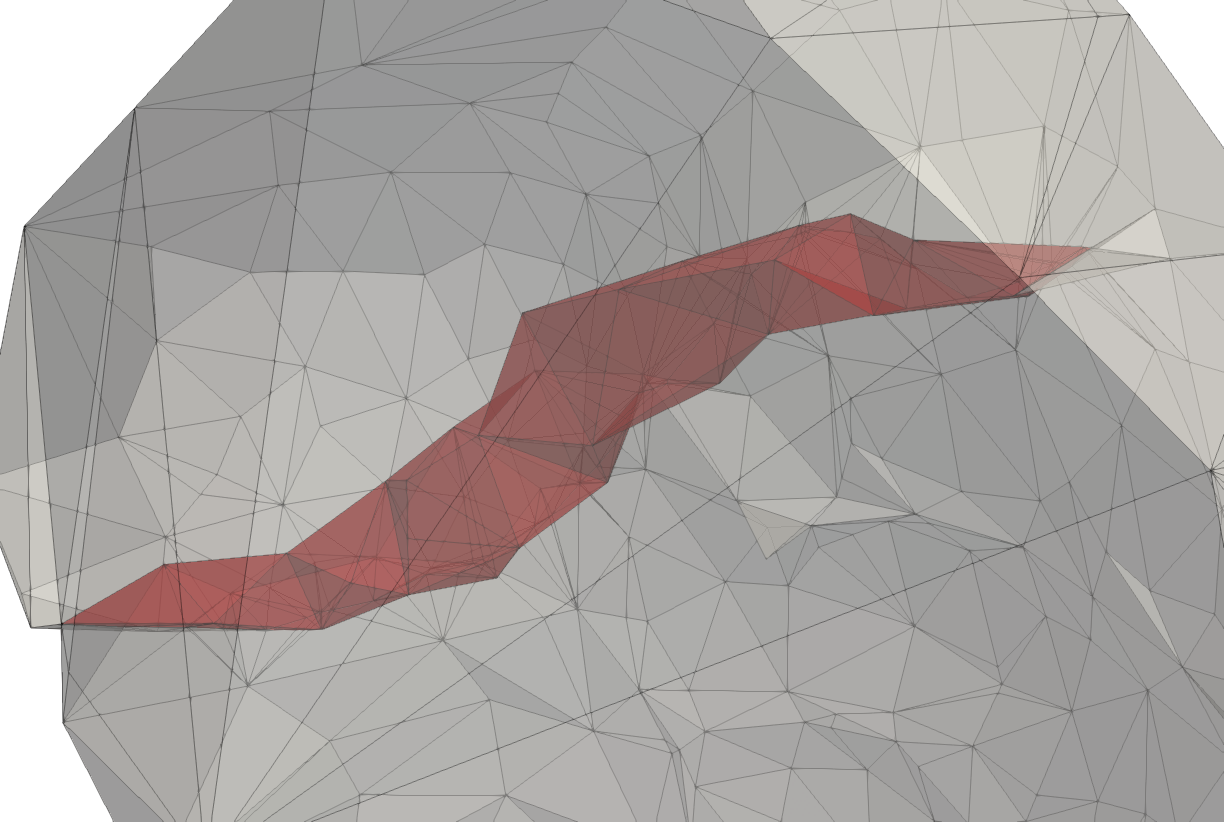
\includegraphics[width=\textwidth]{pics/pic_self_intersection_on.png}
    \caption{The surface before removing the self-intersection.}\label{fig:pic_self_intersection_on}
  \end{minipage}
  \hfill
  \begin{minipage}[h]{0.49\textwidth}
    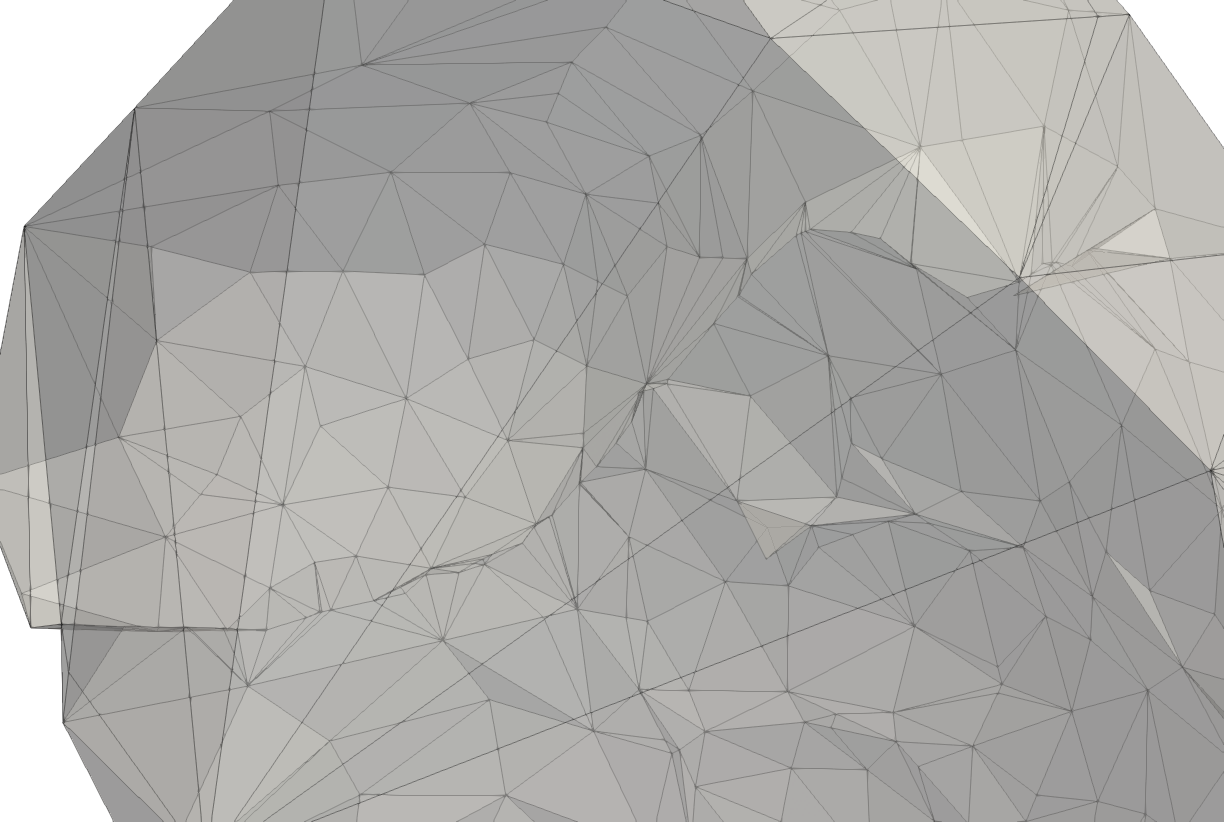
\includegraphics[width=\textwidth]{pics/pic_self_intersection_off.png}
    \caption{The surface after removing the self-intersection.}\label{fig:pic_self_intersection_off}
  \end{minipage}
\end{figure}

\begin{figure}[h]
  \centering
  \begin{minipage}[h]{0.49\textwidth}
    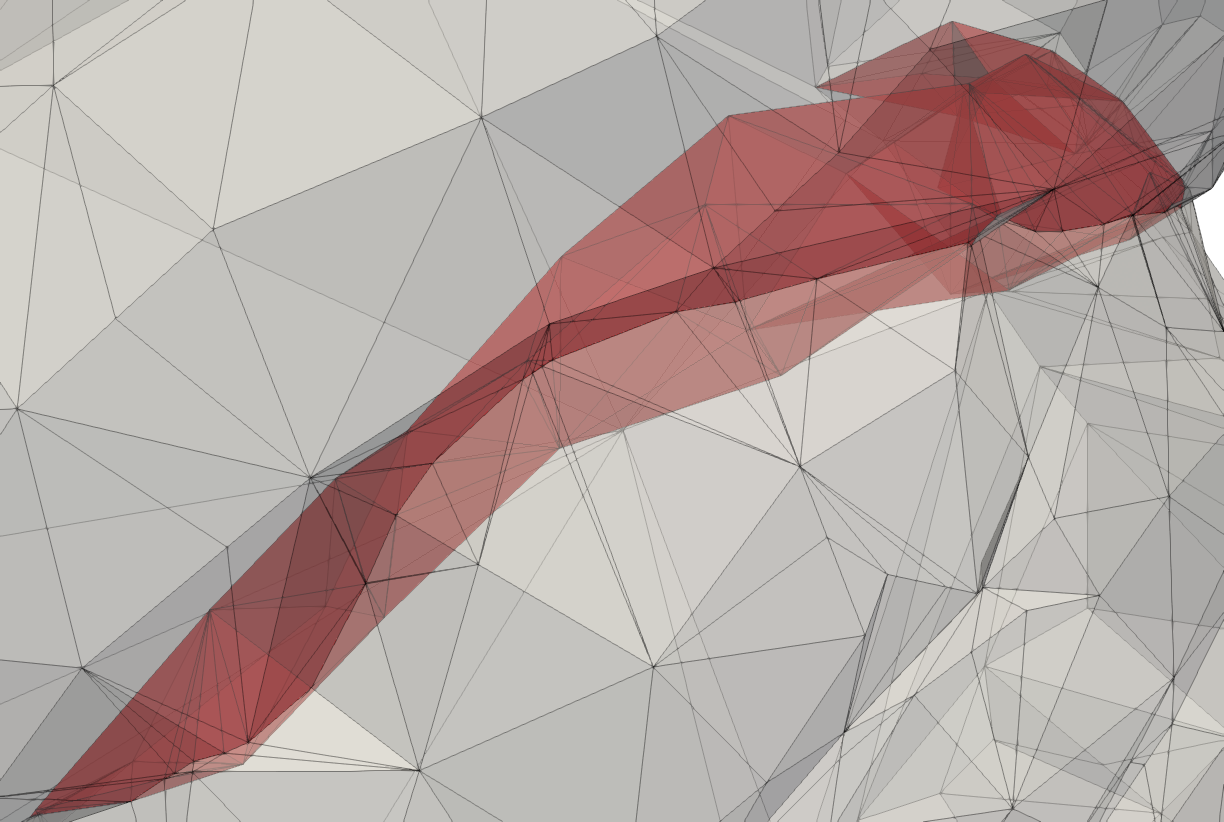
\includegraphics[width=\textwidth]{pics/pic_self_intersection_on_2.png}
    \caption{The surface before removing the self-intersection.}\label{fig:pic_self_intersection_on_2}
  \end{minipage}
  \hfill
  \begin{minipage}[h]{0.49\textwidth}
    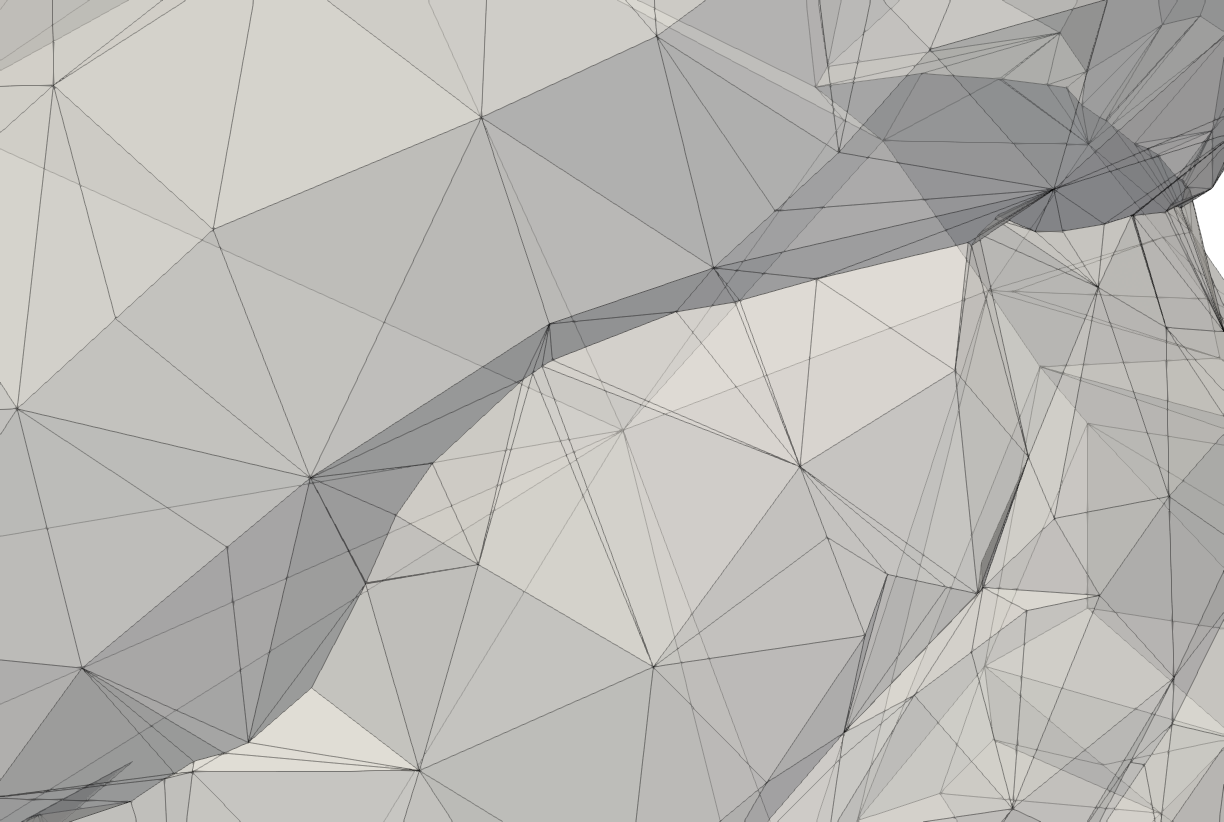
\includegraphics[width=\textwidth]{pics/pic_self_intersection_off_2.png}
    \caption{The surface after removing the self-intersection.}\label{fig:pic_self_intersection_off_2}
  \end{minipage}
\end{figure}

%Объединяя вместе оба рассмотренных случая, получаем критерий выбора следующей для обхода ячейки: должна быть выбрана ячейка, для которой значение показателя $f(P)$ максимально, где
Combining both considered cases together, we obtain a criterion for choosing the next face to bypass: a face must be chosen for which the value of the function $f(P)$ is maximum, where

\begin{equation}
f(P) = 
\begin{cases}
(\vec{n}_A, \vec{OP}), \text{for simple meshes}, \\
-\phi(A \rightarrow P), \text{for general case meshes}
\end{cases}
\end{equation}

%После завершения обхода расчетной сетки все помеченные ячейки считаются ячейками целевой поверхности, а все остальные ячейки должны быть удалены.
After completion of the computational mesh bypass, all marked faces are considered to be faces of the target surface, and all other faces must be deleted.
%На рисунках Fig.~\ref{fig:pic_self_intersection_on} -- Fig.~\ref{fig:pic_self_intersection_off_2} проиллюстрированы примеры устранения самопересечений сетки в виде скрытых петель.
Figures Fig.~\ref{fig:pic_self_intersection_on} -- Fig.~\ref{fig:pic_self_intersection_off_2} illustrate examples of eliminating mesh self-intersections in the form of hidden loops.
%После удаления скрытых ячеек целевая расчетная сетка снова становится корректной, удовлетворяет соотношениям (\ref{eq_arch}) и может быть использована для дальнейшего моделирования ледообразования.
After removing the hidden faces, the target computational mesh again becomes correct, satisfies the relations (\ref{eq_arch}) and can be used for further ice formation modeling.

%---------------------------------------------------------------------------------------------------

\section{Conclusion}

%В статье рассмотрен геометрический аспект задачи моделирования процесса ледообразования, а именно задача эволюции неструктурированной поверхностной расчетной сетки.
The article considers the geometric aspect of the problem of modeling the process of ice formation, namely the problem of the evolution of an unstructured surface computational mesh.
%В процессе эволюции изменение положения узлов сетки должно соответствовать объему накопленного льда в ячейках сетки, а сама сетка должна оставаться корректной, целостной и не содержать самопересечений.
In the process of evolution, the change in the position of the mesh nodes must correspond to the volume of accumulated ice in the mesh faces, and the mesh itself must remain correct, complete, and not contain self-intersections.
%В противном случае продолжение моделирования процесса ледообразования может оказаться невозможным.
Otherwise, it may not be possible to continue modeling the ice formation process.

%Эволюция расчетной сетки состоит из двух основных этапов.
The evolution of the computational mesh consists of two main stages.
%На первом этапе происходит вычисление новых положений узлов сетки в соответствии с объемом накопленного льда.
At the first stage, new positions of mesh nodes are calculated in accordance with the volume of accumulated ice.
%Был рассмотрен ряд наиболее распространенных алгоритмов вычисления новых положений узлов, а также предложен новый алгоритм.
A number of the most common algorithms for calculating new node positions were considered, and a new algorithm was proposed.
%Среди рассмотренных алгоритмов вычисления новых положений узлов присутствовали классические алгоритмы явного вычисления координат узлов, базирующиеся на аппроксимации объема льда в виде простых геометрических фигур (метод призм и метод пирамид).
Among the considered algorithms for calculating new positions of nodes, there were classical algorithms for explicitly calculating the coordinates of nodes, based on the approximation of the ice volume in the form of simple geometric figures (the prisms method and the pyramids method).
%Был рассмотрен многослойный подход, моделирующий итерационное наращивания льда отдельными слоями, позволяющий существенно повысить точность классических методов.
A multilayer approach was considered, which simulates iterative ice growth by separate layers, which makes it possible to significantly improve the accuracy of classical methods.
%Был рассмотрен алгоритм перестроения поверхности, использующий перемещение вершин с сохранением объема, основными особенностями которого являются пошаговое перестроение, вычисление максимальной доли наращиваемого льда для предотвращения локального самопересечения и применение сглаживаний различного вида для эффективной обработки впадин на поверхности тела.
An algorithm for surface rebuilding was considered that uses displacement of vertices while maintaining volume, the main features of which are step-by-step rebuilding, calculation of the maximum proportion of growing ice to prevent local self-intersection, and the use of smoothings of various types to effectively process depressions on the body surface.
%Был предложен новый алгоритм перестроения поверхности, основанный на формировании новой поверхности в виде общей огибающей семейства сфер, центры которых расположены на исходной поверхности, а радиусы соответствует интенсивности нарастания льда.
A new surface rebuilding algorithm was proposed, based on the formation of a new surface in the form of a common envelope of a family of spheres, the centers of which are located on the original surface, and the radiuses correspond to the intensity of ice growth.
%Предложенный алгоритм является линейным по количеству ячеек сетки, устойчивым, а также имеет тенденцию к затягиванию небольших трещин и впадин на поверхности и к сглаживанию острых пиков и изломов.
The proposed algorithm is linear in the number of mesh faces, stable, and also tends to close small cracks and depressions on the surface and smooth out sharp peaks and breaks.

%Так как вне зависимости от применяемого алгоритма перестроения поверхности невозможно дать гарантию отсутствия самопересечения результирующей сетки, то в качестве второго этапа эволюции сетки рассматривалось удаление этих самопересечений.
Since, regardless of the algorithm used for rebuilding the surface, it is impossible to guarantee the absence of self-intersections of the resulting mesh, the removal of these self-intersections was considered as the second stage of mesh evolution.
%Было рассмотрено два подхода к устранению самопересечений.
Two approaches to eliminating self-intersections were considered.
%В основе обоих подходов лежит поиск пересечений ячеек сетки с другими ячейками, отличными от смежных (ячеек пересечения).
Both approaches are based on the search for intersections of mesh faces with other faces other than adjacent ones (crossing faces).
%В основе первого подхода устранения самопересечений является удаление ячеек пересечения с последующим восстановлением сетки.
The first approach to eliminate self-intersections is to remove the intersection faces and then restore.
%В качестве второго подхода рассматривался метод, основанный на дроблении всех ячеек сетки по точкам пересечения с другими ячейками, обходе расчетной сетки начиная со статической области и удаления после данного обхода всех непомеченных ячеек.
As the second approach, we considered a method based on splitting all mesh faces at points of intersection with other faces, bypassing the computational mesh starting from the static area, and removing all unlabeled faces after this bypass.

%Все рассмотренные методы перестроения поверхностей и устранения самопересечений были реализованы и протестированы на предмет применимости в задачах моделирования ледообразования.
All considered methods of rebuilding surfaces and eliminating self-intersections were implemented and tested for applicability in ice formation modeling problems.
%По итогам проведенного тестирования в качестве практического использования был выбран механизм перестроения поверхности, основанный на общей огибающей семейства сфер (так как данный алгоритм является быстрым, надежным и помогает снижать дефекты сетки).
Based on the results of the testing, a surface rebuilding mechanism based on the common envelope of a family of spheres was chosen as a practical use (since this algorithm is fast, reliable, and helps to reduce mesh defects).
%В качестве алгоритма устранения самопересечений сетки предпочтение было отдано алгоритму, основанному на дроблении ячеек по точках пересечения.
As an algorithm for eliminating mesh self-intersections, preference was given to an algorithm based on splitting faces at intersection points.
%Данный алгоритм, хоть и является достаточно медленным (за счет необходимости анализа на пересечение всех потенциально конфликтующих пар ячеек), однако применим к расчетным сеткам произвольной геометрии и сложности.
This algorithm, although rather slow (due to the need to analyze for the intersection of all potentially conflicting pairs of faces), is applicable to computational meshes of arbitrary geometry and complexity.

\begin{acknowledgments}
The work was carried out at the JSCC RAS as part of the government assignment (topic FNEF-2022-0016). Supercomputer MVS-10P was used in research.
\end{acknowledgments}

%---------------------------------------------------------------------------------------------------

\begin{thebibliography}{99}

% Introduction.

\bibitem{Raj}
\refitem{article}
L.~Prince Raj, K.~Yee, and R.~S.~Myong, \textquotedblleft Sensivity of ice and aerodynamic performance degradation to critical physical and modeling parameters affecting airfoil icing,\textquotedblright \ Aerospace Science and Technology, {\bf 98}, 105659 (2020).

\bibitem{Martini}
\refitem{article}
F.~Martini, H.~Ibrahim, L.~T.~C.~Montoya, P.~Rizk, and A.~Ilinca, \textquotedblleft Turbulence modeling of iced wind turbine airfoils,\textquotedblright \ Energies, {\bf 15}, 8325 (2022).

\bibitem{Strijhak}
\refitem{article}
S.~Strijhak, V.~Melnikova, and K.~Koshelev, \textquotedblleft Development of iceFoam solver for modeling ice accretion,\textquotedblright \ in \textit{Proceedings of the Institute for System Programming of RAS, 2020}.

\bibitem{Sorokin}
\refitem{article}
K.~E.~Sorokin, P.~M.~Byvaltsev, A.~A.~Aksenov, S.~V.~Zhluktov, D.~V.~Savitskiy, A.~A.~Babulin, and V.~I.~Shevyakov, \textquotedblleft Numerical simulation of ice accretion if FlowVision sotfware,\textquotedblright \ Computer Research and Modeling, {\bf 12}, №~1, 83--96 (2020).

\bibitem{Galanov}
\refitem{article}
N.~G.~Galanov, A.~V.~Sarazov, R.~N.~Zhukov, and A.~S.~Kozelkov, \textquotedblleft Application of various ice accretion simulation approaches in the LOGOS software package,\textquotedblright \ Journal of Physics: Conference Series, {\bf 2099}, 012029 (2021).

\bibitem{Bartkus}
T.~P.~Bartkus, P.~M.~Struk, and J.-C.~Tsao, \textquotedblleft Evaluation of a thermodynamic ice-crystal icing model using experimental ice accretion data,\textquotedblright \ in \textit{Proceedings of the Atmospheric and Space Environments Conference, 2018}

\bibitem{Zhang}
X.~Zhang, X.~Wu, and J.~Min, \textquotedblleft Aircraft icing model considering both rime ice property variability and runback water effect,\textquotedblright \ International Journal of Heat and Mass Transfer, {\bf 104}, 510--516 (2017).

\bibitem{Pena}
D.~Pena, Y.~Hoarau, and E.~Laurendeau, \textquotedblleft A single step ice accretion model using level-set method,\textquotedblright \ Journal of Fluids and Structures, {\bf 65}, 278--294 (2016).


% Remesh.

\bibitem{Beaugendre}
\refitem{misc}
H.~Beaugendre, \textquotedblleft A PDE-based approach to in-flight ice accretion,\textquotedblright \ PhD Thesis (Dep. of Mech. Eng., McGill Univ., Montr\'eal, Qu\'ebec, 2003).

\bibitem{Rybakov_2D}
\refitem{article}
A.~Rybakov and S.~Shumilin, \textquotedblleft Approximate methods of the surface mesh deformation in two-dimensional case,\textquotedblright \ Lobachevskii J Math {\bf 40}, 1848--1852 (2019).

\bibitem{BourgaultCote}
\refitem{article}
S.~Bourgault-C\^ot\'e, K.~Hasanzadeh, P.~Lavoie, and E.~Laurendeau, \textquotedblleft Multi-layer icing methodologies for conservative ice growth,\textquotedblright \ in \textit{Proceedings of 7th European Conference for Aeronautics and Aerospace Sciences EUCASS, 2017}.

\bibitem{Thompson}
\refitem{article}
D.~Thompson, X.~Tong, Q.~Arnoldus, E.~Collins, D.~McLaurin, and E.~Luke, \textquotedblleft Discrete surface evolution and mesh deformation for aircraft icing applications,\textquotedblright \ in \textit{Proceedings of the 5th AIAA Atmospheric and Space Environments Conference, 2013}.

\bibitem{Tong}
\refitem{article}
X.~Tong, D.~Thompson, Q.~Arnoldus, E.~Collins, and E.~Luke, \textquotedblleft Three-dimensional surface evolution and mesh deformation for aircraft icing applications,\textquotedblright \ Journal of Aircraft, {\bf 54}, 1047--1063 (2017).

\bibitem{Jiao}
\refitem{article}
X.~Jiao, \textquotedblleft Face offsetting: a unified approach for explicit moving interfaces,\textquotedblright \ Journal of Computational Physiscs, {\bf 220}, 612--625 (2007).

\bibitem{Jiao_null_space_smooth}
\refitem{article}
X.~Jiao, \textquotedblleft Volume and feature preservation in surface mesh optimization,\textquotedblright \ in \textit{Proceedings of the 15th International Meshing Roundtable, 2006}.

% Adaptation.

\bibitem{Rivara}
\refitem{article}
M.-C.~Rivara and P.~A.~Rodrigez-Moreno, \textquotedblleft Tuned terminal triangles centroid Delaunay algorithm for quality triangulation,\textquotedblright \ in \textit{27th International Meshing Roundtable, 2019}.

\bibitem{Rakotoarivelo}
\refitem{article}
H.~Rakotoarivelo and F.~Ledoux, \textquotedblleft Accurate manycore-accelerated manifold surface remesh kernels,\textquotedblright \ in \textit{27th International Meshing Roundtable, 2019}.

\bibitem{Borouchaki}
\refitem{article}
H.~Borouchaki, P.~Laug, and P.-L.~George, \textquotedblleft Parametric surface meshing using a combined advancing-front generalized Delaunay approach,\textquotedblright \ International Journal for Numerical Methods in Engineering, {\bf 49}, 233--259 (2000).

\bibitem{Panchal}
\refitem{article}
D.~Panchal and D.~Jayaswal, \textquotedblleft Feature sensitive geometrically faithful highly regular direct triangular isotropic surface remeshing,\textquotedblright \ S$\bar{a}$dhan$\bar{a}$, {\bf 47}, 94 (2022).

% SLE

\bibitem{Jung}
\refitem{article}
W.~Jung, H.~Shin, and B.~K.~Choi, \textquotedblleft Self-intersection removal in triangular mesh offsettings,\textquotedblright \ CAD Journal, {\bf 1}, № 1, 477--484 (2004).

\bibitem{Freylekhman}
\refitem{article}
S.~A.~Freylekhman and A.~A.~Rybakov, \textquotedblleft Self-intersection elimination for unstructured surface computational meshes,\textquotedblright \ Lobachevskii J Math {\bf 43}, 134--140 (2022).

\bibitem{Charton}
\refitem{article}
J.~Charton, S.~Baek, and Y.~Kim, \textquotedblleft Mesh repairing using topology graphs,\textquotedblright \ Journal of Computational Design and Engineering, {\bf 8}, 251--267 (2021).

\bibitem{Skvorkovska}
\refitem{article}
V.~Skorkovsk\'a, I.~Kolingerov\'a, and B.~Benes, \textquotedblleft A Simple and robust approach to computation of meshes intersection,\textquotedblright \ in \textit{Proceedings of the 13th International Joint Conference on Computer Vision, Imaging and Computer Graphics Theory and Applications, {\bf 1}, 175--182, 2018}.

\end{thebibliography}

\end{document}
